% Created 2024-11-25 Mon 22:54
% Intended LaTeX compiler: pdflatex
\documentclass[11pt]{article}
\usepackage[utf8]{inputenc}
\usepackage[T1]{fontenc}
\usepackage{graphicx}
\usepackage{longtable}
\usepackage{wrapfig}
\usepackage{rotating}
\usepackage[normalem]{ulem}
\usepackage{amsmath}
\usepackage{amssymb}
\usepackage{capt-of}
\usepackage{hyperref}
\usepackage{minted}
\usepackage{siunitx}
\usepackage{mathtools}
\setlength{\parindent}{0em}
\author{Hankertrix}
\date{\today}
\title{MA1001 Dynamics Cheat Sheet}
\hypersetup{
 pdfauthor={Hankertrix},
 pdftitle={MA1001 Dynamics Cheat Sheet},
 pdfkeywords={},
 pdfsubject={},
 pdfcreator={Emacs 29.4 (Org mode 9.6.15)}, 
 pdflang={English}}
\begin{document}

\maketitle
\setcounter{tocdepth}{2}
\tableofcontents \clearpage
\section{Definitions}
\label{sec:orgf8e7da4}

\subsection{Scalars}
\label{sec:org70d8fc7}
Scalars are quantities that are fully described by a \textbf{magnitude} (or numerical value) alone, like mass, length, time, and energy.

\subsection{Vectors}
\label{sec:org7988219}
Vectors are quantities that are fully described by both a \textbf{magnitude} and a \textbf{direction}, like displacement, velocity and acceleration.

\subsection{Rectilinear motion}
\label{sec:org4fdc5ce}
Rectilinear motion is defined as the motion of a particle along a straight line.

\subsection{Position coordinates}
\label{sec:orgc63e0c6}
The position coordinates is the coordinates that wholly defines the position of a particle, usually from an origin.

\subsection{Reference frames}
\label{sec:orgfe21654}
Reference frames are the frames in which a coordinate system is created to determine an object's motion.

\subsubsection{Absolute reference frame}
\label{sec:org13d2412}
The absolute reference frame is the frame that never moves. In other words, it is glued to the ground and does not translate or rotate as the ground never moves.

\subsubsection{Point-attached reference frame}
\label{sec:org64cca16}
Point-attached reference frames are reference frames that are attached to a point on an object or body. These reference frames never rotate, only translate. The origin of the reference frame is the point the reference frame is attached to. In other words, the origin of a point-attached reference frame is glued to a point on an object or a body, and since a point cannot be rotated, the reference frame likewise also cannot be rotated, only translated.

\subsubsection{Body-attached reference frame}
\label{sec:org211eec8}
Body-attached reference frames are reference frames where the reference frame is attached to an object or body. The reference frame can be thought of as being glued to an object or body. Such reference frames can both translate and rotate, as they follow the body's motion.

\subsection{Velocity (\(v\))}
\label{sec:org1baa9a5}
The velocity of a particle is equal to the time derivative of the particle's position (\(x\)), i.e.
\[v = \frac{dx}{dt}\]

Where:
\begin{itemize}
\item \(v\) is the velocity of the particle
\item \(\frac{dx}{dt}\) is the derivative of the position of the particle with respect to time
\end{itemize}

\subsection{Acceleration (\(a\))}
\label{sec:org4ccc392}
The acceleration of a particle is obtained by differentiating the particle's velocity (\(v\)) with respect to time, i.e.
\[a = \frac{dv}{dt}\]
\[a = \frac{d^2x}{dt^2}\]
\[a = v \frac{dv}{dx}\]

Where:
\begin{itemize}
\item \(a\) is the acceleration of the particle
\item \(\frac{dv}{dt}\) is the derivative of the velocity of the particle with respect to time
\item \(\frac{d^2x}{dt^2}\) is the second derivative of the position of the particle with respect to time
\item \(v\) is the velocity of the particle
\item \(\frac{dv}{dx}\) is the derivative of the velocity of the particle with respect to its position
\end{itemize}

\subsection{Right-hand grip (screw) rule}
\label{sec:org90eb84e}
\begin{center}
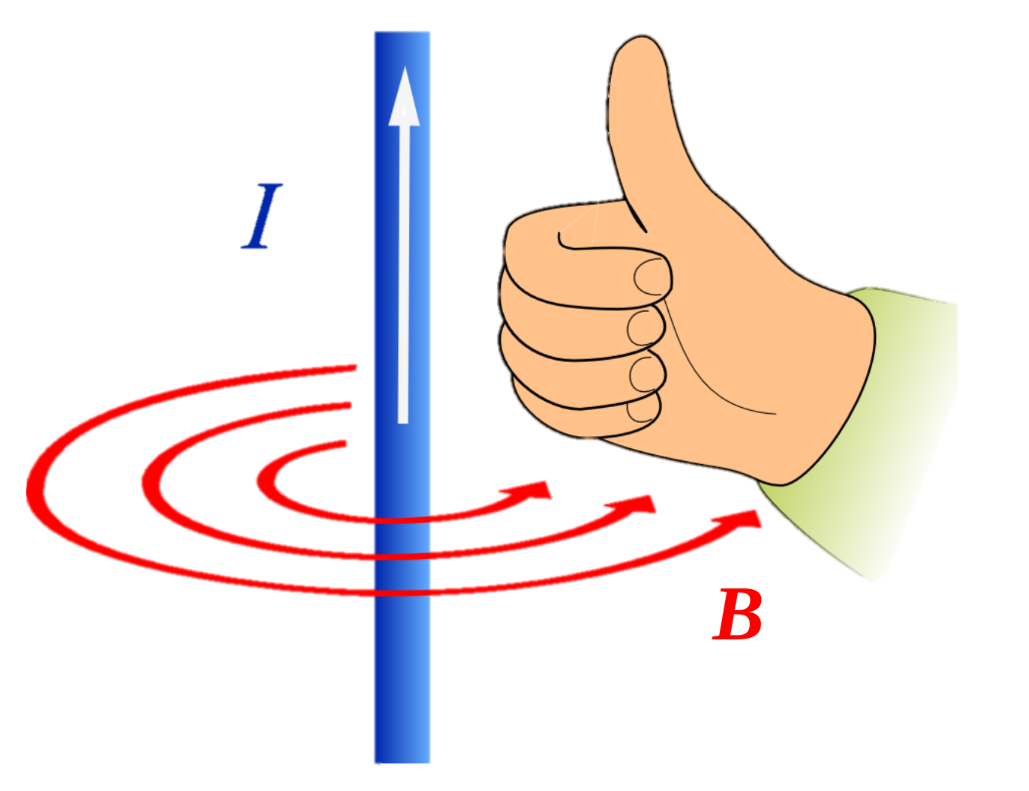
\includegraphics[width=.9\linewidth]{./images/right-hand-grip-rule.png}
\end{center}

\subsection{Circular motion}
\label{sec:orgea54ba8}

\subsubsection{Period (\(T\))}
\label{sec:org339ba01}
Period refers to the time taken for an object in circular motion to complete one revolution.

\subsubsection{Frequency (\(f\))}
\label{sec:orgb0f3c5e}
\[f = \frac{1}{T}\]

Where:
\begin{itemize}
\item \(f\) is the frequency
\item \(T\) is the period
\end{itemize}

 \newpage

\subsubsection{Angular displacement (\(\theta\))}
\label{sec:org0af97bf}
\[\theta = \frac{\text{Arc length}}{r}\]

Where:
\begin{itemize}
\item \(\theta\) is the angular displacement of the object in circular motion
\item \(r\) is the distance of the object from the centre of the circle
\end{itemize}

\subsubsection{Angular velocity (\(\vec{\omega}\))}
\label{sec:org614a8b3}
\[\vec{\omega} = \frac{2 \pi}{T} \hat{e}\]
\[\vec{\omega} = \frac{\theta}{t} \hat{e}\]
\[\vec{\omega} = \frac{\vec{v}}{r}\]

Where:
\begin{itemize}
\item \(\vec{\omega}\) is the angular velocity vector of the object in circular motion
\item \(T\) is the period
\item \(\theta\) is the angle rotated by the object in circular motion
\item \(t\) is the time taken for the object to rotate the angle \(\theta\)
\item \(\hat{e}\) is the direction vector perpendicular to the plane that the motion is taking place, usually \(\vec{k}\). Use the right-hand grip (screw) rule to figure out the direction of the angular velocity.
\item \(\vec{v}\) is the velocity vector of the object in circular motion
\item \(r\) is the distance of the object from the centre of the circle
\end{itemize}

 \newpage

\subsubsection{Angular acceleration (\(\vec{\alpha}\))}
\label{sec:org0981021}
\[\vec{\alpha} = \frac{a_t}{r} \hat{e}\]
\[\vec{\alpha} = \frac{\vec{\omega}}{t}\]

Where:
\begin{itemize}
\item \(\vec{\alpha}\) is the angular acceleration of the object in circular motion
\item \(a_t\) is the magnitude of the tangential acceleration of the object in circular motion
\item \(\hat{e}\) is the direction vector perpendicular to the plane that the motion is taking place, usually \(\vec{k}\). Use the right-hand grip (screw) rule to figure out the direction of the angular velocity.
\item \(r\) is the distance of the object from the centre of the circle
\item \(\vec{\omega}\) is the angular velocity of the object in circular motion
\item \(t\) is the time taken for the object to rotate
\end{itemize}

\subsubsection{Position (\(\vec{r}\))}
\label{sec:orge76ac7c}
\[\vec{r} = r_0 \vec{e}_r = r_0 (\cos \theta \hat{i} + \sin \theta \hat{j})\]

Where:
\begin{itemize}
\item \(\vec{r}\) is the position vector of an object in circular motion
\item \(r_0\) is the distance of the object away from the centre of the circle
\item \(\theta\) is the angular displacement
\end{itemize}

 \newpage

\subsubsection{Velocity (\(\vec{v}\))}
\label{sec:orga4d2a3d}
\[\vec{v} = \frac{d \vec{r}}{dt} = \frac{d}{dt} (r_0 \hat{e}_r) = r_0 \frac{d \hat{e}_r}{dt}\]
\[\frac{d \hat{e}_r}{dt} = \dot{\theta} (- \sin \theta \hat{i} + \cos \theta \hat{j}) = \omega \hat{e}_{\theta}\]
\[\vec{v} = \vec{\omega} \times \vec{r}\]

Where:
\begin{itemize}
\item \(\vec{v}\) is the velocity vector of the object in circular motion
\item \(r_0\) is the distance of the object from the centre of the circle
\item \(\hat{e}_r\) is the unit vector parallel to the position vector of the object
\item \(\dot{\theta}\) is the rate of change of angular displacement
\item \(\theta\) is the angular displacement
\item \(\hat{e}_{\theta}\) is the unit vector perpendicular to the position vector of the object, it is \(\hat{e}_r\) rotated \(90^{\circ}\) anti-clockwise
\item \(\vec{\omega}\) is the angular velocity vector of the object
\item \(\vec{r}\) is the position vector of the object with respect to the centre of the circle, i.e. the centre of the circle is the origin
\end{itemize}

\subsubsection{Tangential acceleration (\(\vec{a}_t\))}
\label{sec:orgebc62dc}
Tangential acceleration of an object in circular motion is the acceleration \textbf{parallel} to its direction of motion. Tangential acceleration only changes the \textbf{speed} or the \textbf{magnitude of the velocity} of the object.
\[\vec{a}_t = \vec{\alpha} \times \vec{r}\]

Where:
\begin{itemize}
\item \(\vec{a}\) is the tangential acceleration vector of the object in circular motion
\item \(\vec{\alpha}\) is the angular acceleration vector of the object
\item \(\vec{r}\) is the position vector of the object with respect to the centre of the circle, i.e. the centre of the circle is the origin
\end{itemize}

 \newpage

\subsubsection{Centripetal or normal acceleration (\(\vec{a}_n\))}
\label{sec:org0ee6996}
Centripetal or normal acceleration of an object in circular motion is the acceleration \textbf{perpendicular} to its direction of motion. Centripetal or normal acceleration only changes the \textbf{direction} of the object.
\[\vec{a}_n = \vec{\omega} \times \vec{v} = - \omega^2 \vec{r} = - \frac{v^2}{r} \hat{e}_{\theta}\]

Where:
\begin{itemize}
\item \(\vec{a}_n\) is the centripetal or normal acceleration of the object in circular motion
\item \(\vec{\omega}\) is the angular velocity vector of an object in circular motion
\item \(\vec{v}\) is the velocity vector of the object in circular motion
\item \(\omega\) is the magnitude of the angular velocity of an object in circular motion
\item \(\vec{r}\) is the position vector of the object with respect to the centre of the circle, i.e. the centre of the circle is the origin
\item \(v\) is the magnitude of the velocity vector
\item \(\hat{e}_{\theta}\) is the unit vector perpendicular to the position vector of the object, it is \(\hat{e}_r\) rotated \(90^{\circ}\) anti-clockwise
\end{itemize}

\subsubsection{Total acceleration (\(\vec{a}\))}
\label{sec:orgcd4efcb}
\[\vec{a} = \vec{a}_t + \vec{a}_n\]

Where:
\begin{itemize}
\item \(\vec{a}\) is the total acceleration of the object in circular motion
\item \(\vec{a}_t\) is the tangential acceleration of the object in circular motion
\item \(\vec{a}_n\) is the centripetal or normal acceleration of the object in circular motion
\end{itemize}

\subsubsection{Physical meaning of the components of total acceleration}
\label{sec:org6f92c5e}
\begin{center}
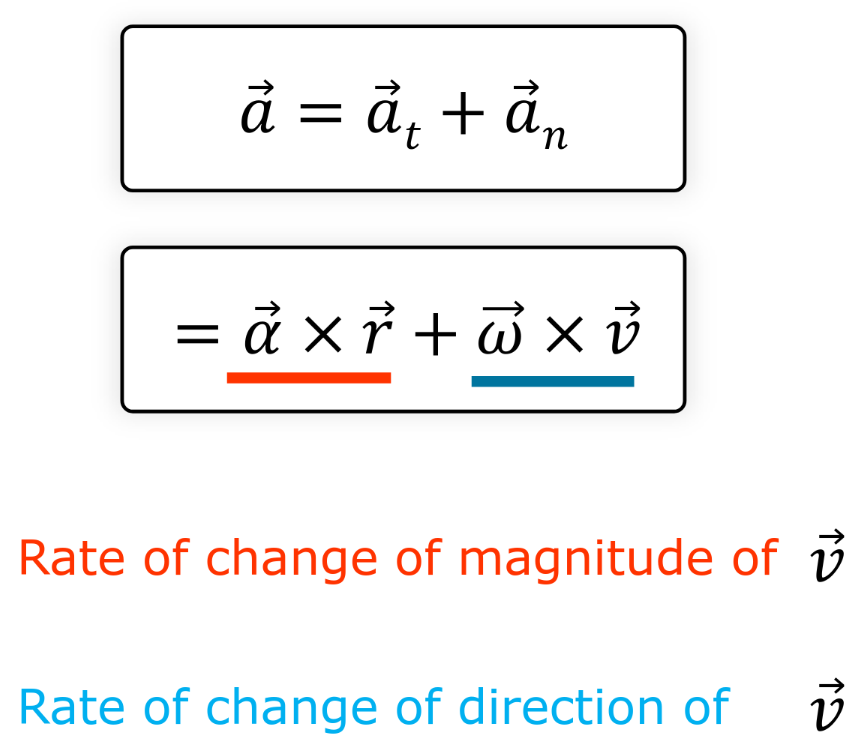
\includegraphics[width=.9\linewidth]{./images/physical-meaning-of-components-of-total-acceleration.png}
\end{center}

 \newpage

\subsection{Uniform rectilinear motion}
\label{sec:orgd4a56ae}
The velocity of the particle is \textbf{constant} in uniform rectilinear motion, i.e.
\[x = x_0 + vt\]

Where:
\begin{itemize}
\item \(x\) is the final position of the particle
\item \(x_0\) is the initial position of the particle
\item \(v\) is the velocity of the particle
\item \(t\) is the time taken by the particle
\end{itemize}

\subsection{Uniformly accelerated rectilinear motion}
\label{sec:org6b19c2b}
The acceleration of the particle is \textbf{constant} in uniformly accelerated rectilinear motion, i.e.
\[v = v_0 + at\]
\[x = x_0 + v_0t + \frac{1}{2}at^2\]
\[v^2 = v_0^2 + 2a(x - x_0)\]

Where:
\begin{itemize}
\item \(v\) is the final velocity of the particle
\item \(x\) is the final position of the particle
\item \(a\) is the acceleration of the particle
\item \(t\) is the time take by the particle
\item \(v_0\) is the initial velocity of the particle
\item \(x_0\) is the initial position of the particle
\end{itemize}

 \newpage

\subsection{Acceleration of free fall}
\label{sec:org4b8f170}
The acceleration of free fall is \(\qty{-9.81}{m.s^{-2}}\), taking upwards as positive.

\subsection{Graphical solution}
\label{sec:org68da30d}
\begin{itemize}
\item A graphical solution is essentially just drawing a graph to solve a dynamics problem.
\item A graphical solution most commonly involves:
\begin{itemize}
\item \(x\) - \(t\) curve or displacement-time curve
\item \(v\) - \(t\) curve or velocity-time curve
\item \(a\) - \(t\) curve or acceleration-time curve
\end{itemize}
\item At any given time \(t\):
\begin{itemize}
\item \(v =\) slope of \(x\) - \(t\) curve
\item \(a =\) slope of \(a\) - \(t\) curve
\end{itemize}
\item Over any given time interval \(t_1\) to \(t_2\):
\begin{itemize}
\item \(v_2 - v_1 =\) area under \(a\) - \(t\) curve \(= \int_{t_1}^{t_2} a \, dt\)
\item \(x_2 - x_1 =\) area under \(v\) - \(t\) curve \(= \int_{t_1}^{t_2} v \, dt\)
\end{itemize}
\end{itemize}

 \newpage

\subsection{Curvilinear motion}
\label{sec:orgf8e96f3}
\begin{center}
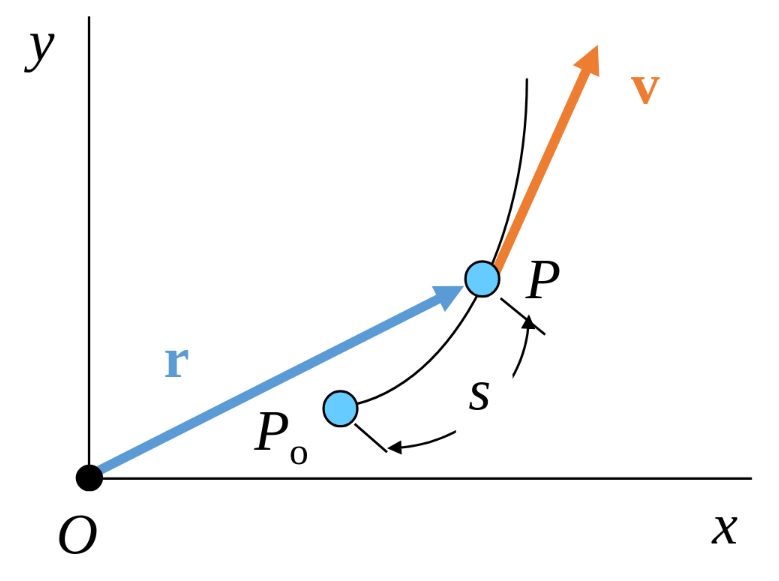
\includegraphics[width=.9\linewidth]{./images/curvilinear-motion-of-particle.png}
\end{center}

The curvilinear motion of a particle involves particle motion along a curved path. The position \(P\) of the particle at a given time is defined by the position vector \(\vec{r}\) joining the origin \(O\) of the coordinate system with the point \(P\).

\subsection{Velocity of a particle in curvilinear motion (\(\vec{v}\))}
\label{sec:org0fa8194}
\begin{center}
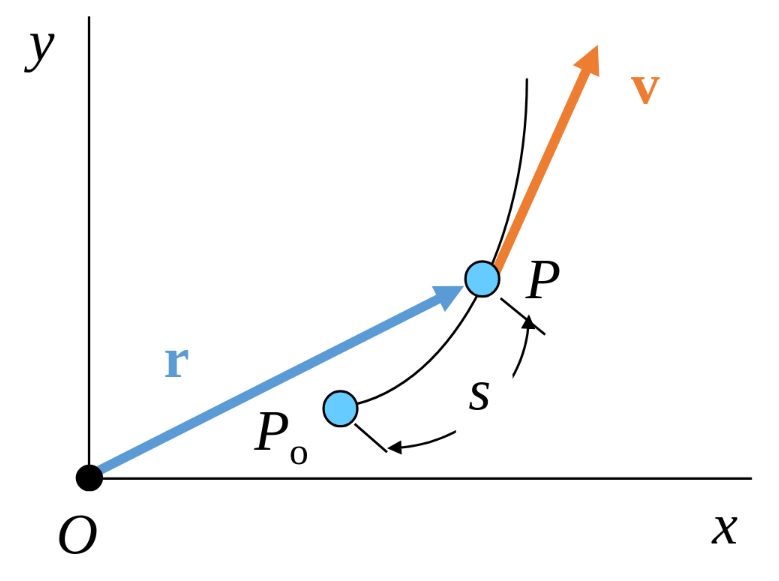
\includegraphics[width=.9\linewidth]{./images/curvilinear-motion-of-particle.png}
\end{center}

The velocity \(\vec{v}\) of the particle is defined by the relation:
\[\vec{v} = \frac{d \vec{r}}{dt}\]

The velocity vector is tangent to the path of the particle, and has a magnitude \(v\) equal to the time derivative of the length \(s\) of the arc described by the particle:
\[v = \frac{ds}{dt}\]

\subsection{Instantaneous velocity of a particle in curvilinear motion (\(\vec{v}_{instant}\))}
\label{sec:org642e38c}
\begin{center}
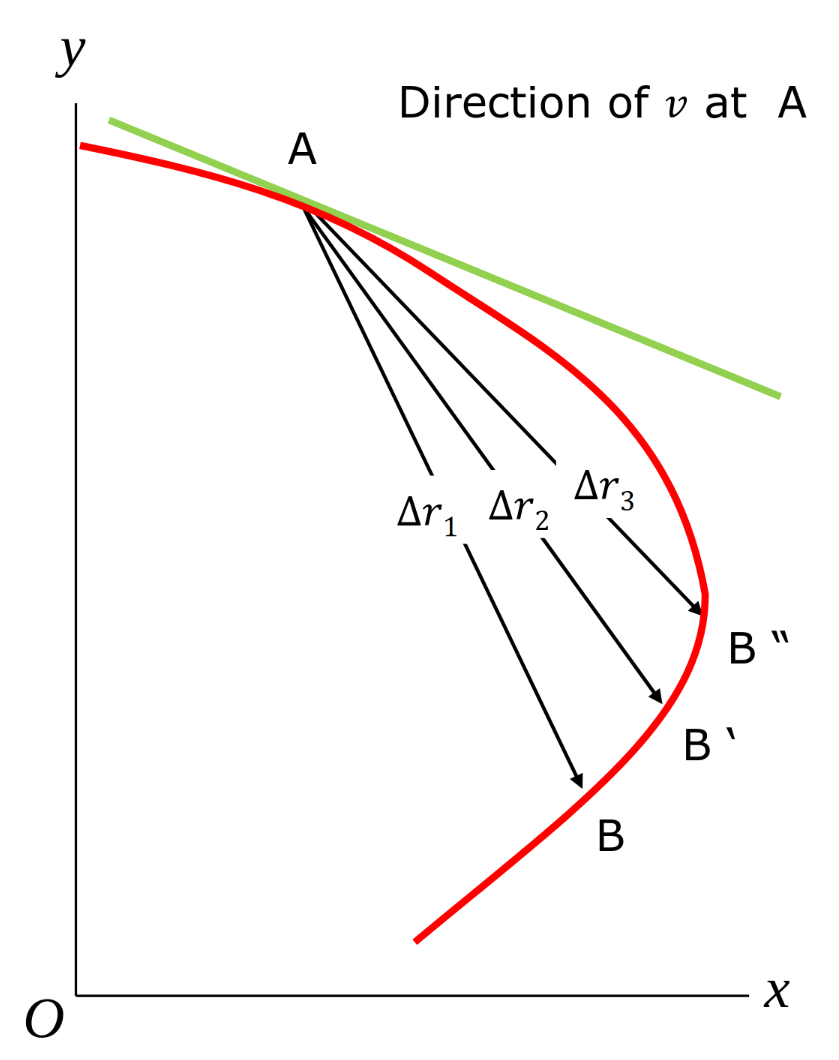
\includegraphics[scale=0.6]{./images/instantaneous-velocity-in-curvilinear-motion.png}
\end{center}

\[\vec{v}_{instant} \equiv \lim_{\Delta t \rightarrow 0} \frac{\Delta \vec{r}}{\Delta t} = \frac{d \vec{r}}{dt}\]

Where:
\begin{itemize}
\item \(\vec{v}_{instant}\) is the instantaneous velocity of the particle in curvilinear motion
\item \(\delta \vec{r}\) is the change in position vector of the particle
\item \(\delta t\) is the change in time
\item \(d \vec{r}\) is the change in position vector of the particle
\item \(dt\) is the infinitesimal change in time
\end{itemize}

\subsection{Acceleration of a particle in curvilinear motion (\(\vec{a}\))}
\label{sec:orgfa3b5eb}
In general, the acceleration \(\vec{a}\) of the particle is not tangent to the \textbf{path of the particle}. It is defined by the relation:
\[\vec{a} = \frac{d \vec{v}}{dt}\]

Where:
\begin{itemize}
\item \(\vec{a}\) is the acceleration vector of the particle
\item \(d \vec{v}\) is the change in the velocity vector
\item \(dt\) is the change in time
\end{itemize}

\subsection{Instantaneous acceleration of a particle in curvilinear motion (\(\vec{a}_{instant}\))}
\label{sec:orga6dff96}
In general, the acceleration \(\vec{a}\) of the particle is not tangent to the \textbf{path of the particle}. It is defined by the relation:

\[\vec{a}_{instant} \equiv \lim_{\Delta t \rightarrow 0} \frac{\Delta \vec{v}}{\Delta t} = \frac{d \vec{v}}{dt}\]

The instantaneous acceleration is the limit of the average acceleration \(\frac{\Delta \vec{v}}{\Delta t}\), as \(\Delta t\) approaches 0.
\begin{itemize}
\item The magnitude of the velocity vector may change.
\item The direction of the velocity vector may change, even if the magnitude remains constant.
\item Both may change simultaneously.
\end{itemize}

Where:
\begin{itemize}
\item \(\vec{a}_{instant}\) is the instantaneous acceleration vector of the particle
\item \(\Delta \vec{v}\) is the change in the velocity vector
\item \(\Delta t\) is the change in time
\item \(d \vec{v}\) is the change in the velocity vector
\item \(dt\) is the infinitesimal change in time
\end{itemize}

\subsection{Rectangular coordinate system}
\label{sec:org0bb07fc}
Denoting \(x, y\) and \(z\) as the rectangular coordinates of a particle \(P\), the rectangular components of velocity and acceleration of \(P\) are equal to the first and second derivatives with respect to \(t\) of the corresponding coordinates:
\begin{center}
\begin{tabular}{ c c c }
$v_x = \dot{x}$ & $v_y = \dot{y}$ & $v_z = \dot{z}$ \\
$a_x = \ddot{x}$ & $a_y = \ddot{y}$ & $a_z = \ddot{z}$
\end{tabular}
\end{center}

The use of rectangular components is particularly effective in the study of the motion of particles.

\subsection{Path coordinate system}
\label{sec:orgdfaf524}
\begin{center}
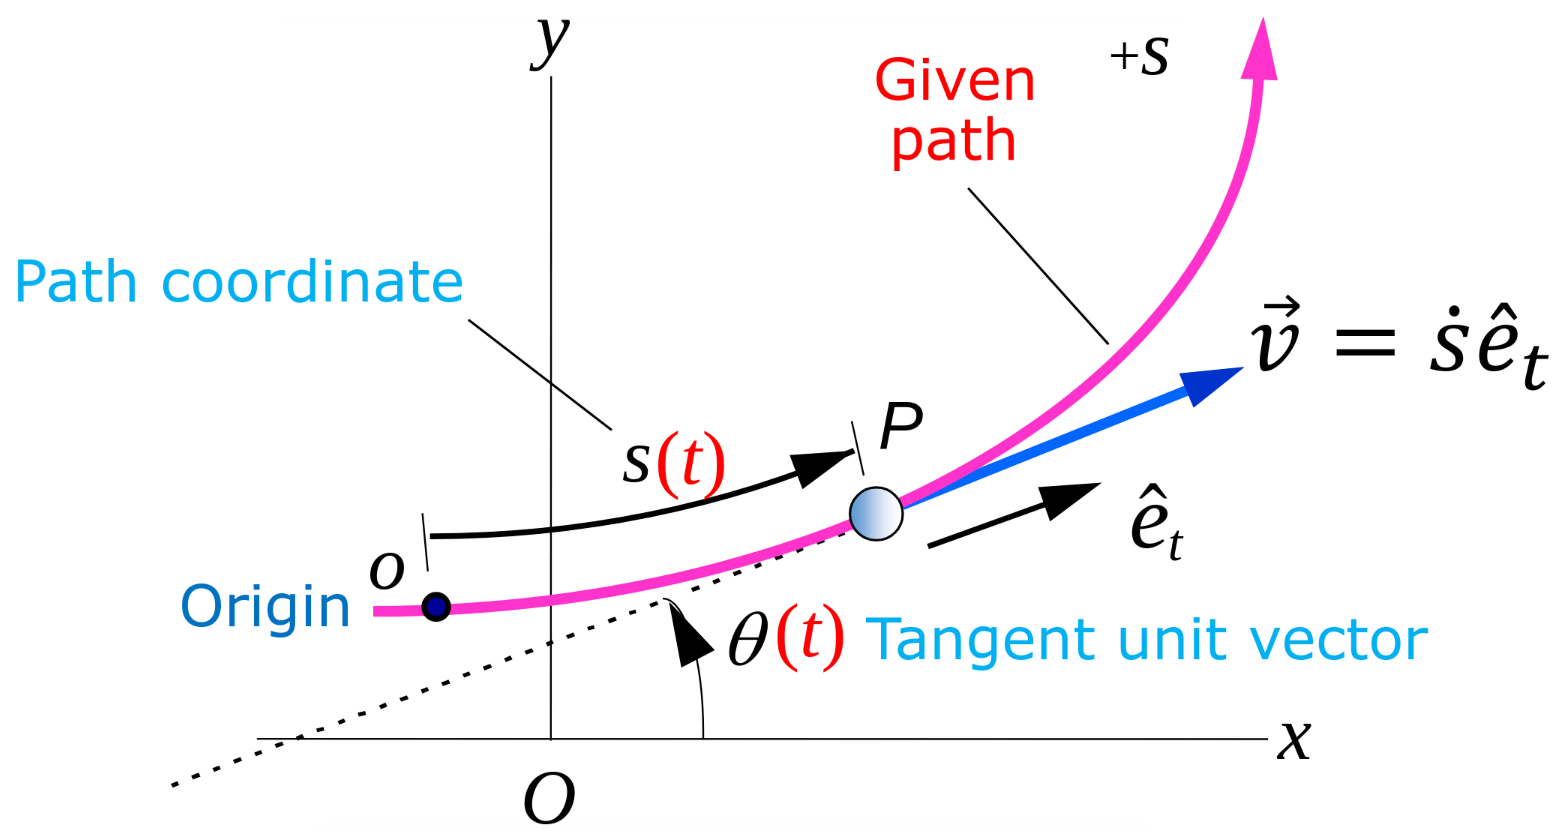
\includegraphics[width=.9\linewidth]{./images/path-coordinate-system.png}
\end{center}

\[\hat{e}_t = \cos \theta (t) \hat{i} + \sin \theta (t) \hat{j}\]
\[\vec{v} = \dot{s} \hat{e}_t = v \hat{e}_t = v \angle \theta = \dot{s} \theta\]

Where:
\begin{itemize}
\item \(\hat{e}_t\) is the unit vector directed along the tangent to the path
\item \(\theta (t)\) is the tangent unit vector
\item \(\vec{v}\) is the velocity vector directed along the tangent to the path
\item \(\dot{s}\) is the rate of change of the path coordinate
\item \(v\) is the speed of the particle
\end{itemize}

\subsubsection{Kinematics equations}
\label{sec:org76a98de}
\begin{center}
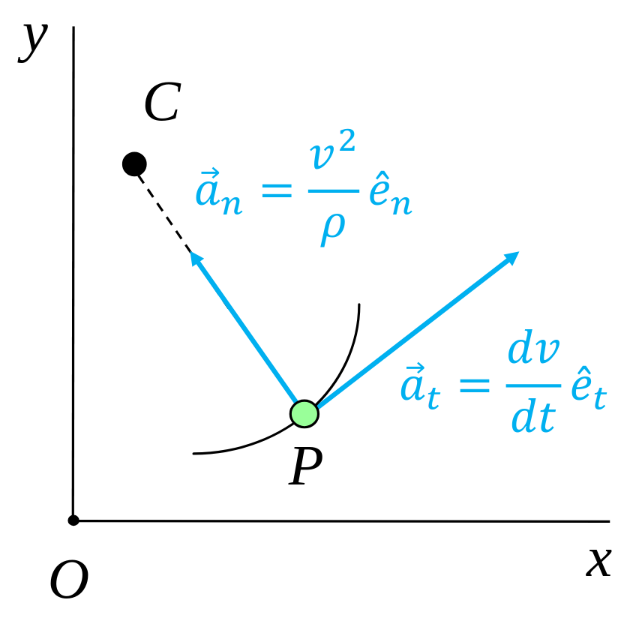
\includegraphics[width=.9\linewidth]{./images/path-coordinates-kinematics-equations.png}
\end{center}
\[\vec{v} = v \hat{e}_t\]
\[\vec{a} = \frac{dv}{dt} \hat{e}_t + \frac{v^2}{\rho} \hat{e}_n\]

Where:
\begin{itemize}
\item \(\vec{v}\) is the velocity vector directed along the tangent to the path
\item \(v\) is the speed of the particle
\item \(\hat{e}_t\) is the unit vector directed along the tangent to the path
\item \(\rho\) is the radius of curvature of its path.
\item \(\vec{a}\) is the acceleration vector
\item \(\hat{e}_n\) is the unit vector directed towards the centre of curvature of the path
\end{itemize}

\subsubsection{Radius of curvature (\(\rho\))}
\label{sec:orgfa18822}
\begin{center}
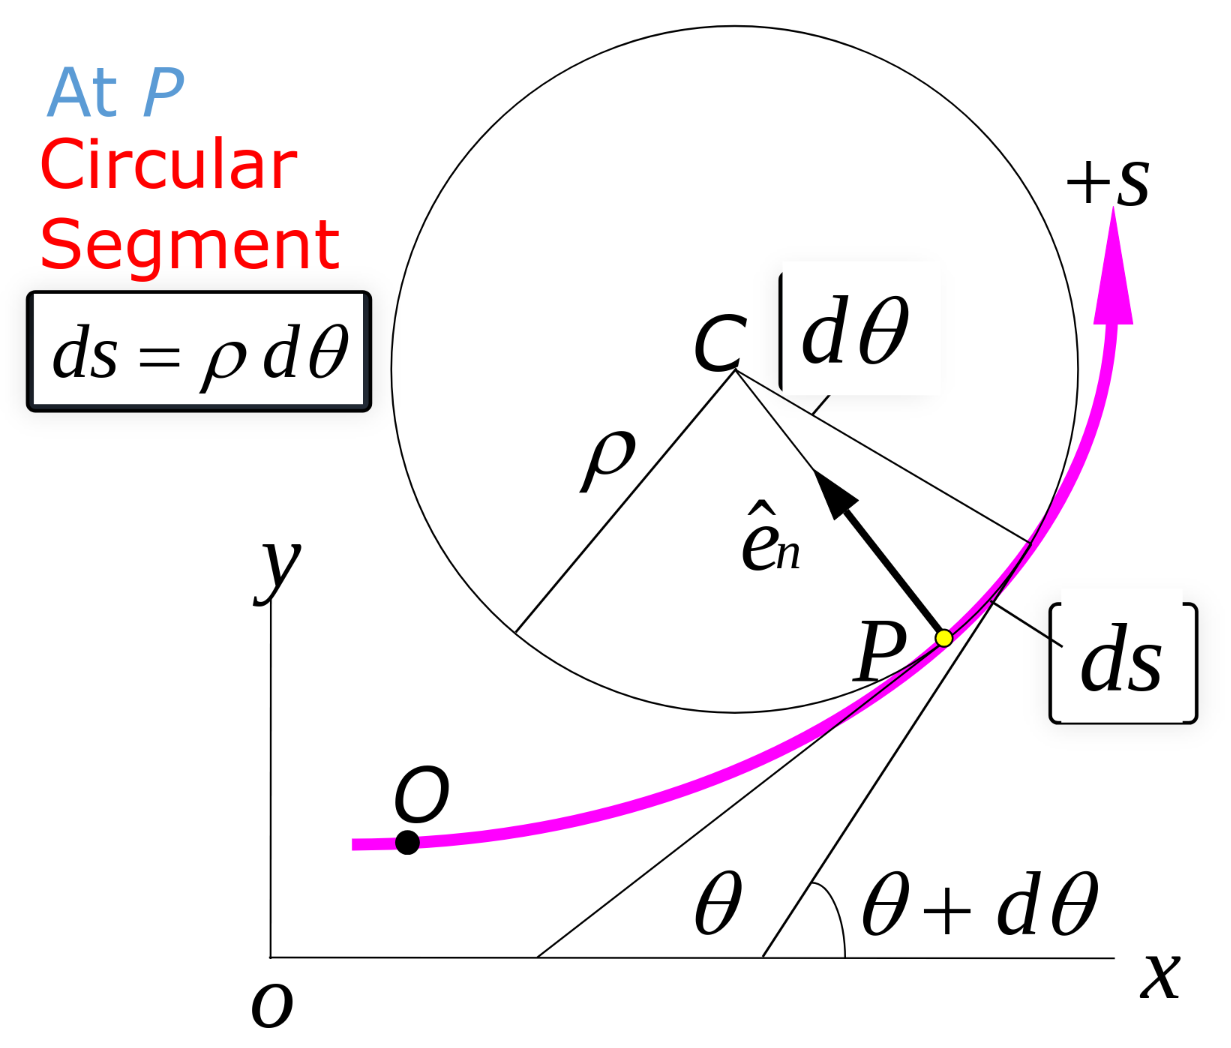
\includegraphics[width=.9\linewidth]{./images/radius-of-curvature-in-path-coordinate-system.png}
\end{center}
\[\rho = \lim_{\Delta \theta \rightarrow 0} \left|\frac{\Delta s}{\Delta \theta} \right| = \left| \frac{ds}{d \theta} \right| = \left| \frac{\frac{ds}{dt}}{\frac{d \theta}{dt}} \right| = \left| \frac{v}{\omega} \right|\]

Where:
\begin{itemize}
\item \(\rho\) is the radius of curvature
\item \(\Delta s\) is the change in path coordinate
\item \(\Delta \theta\) is the change in angle subtended from the middle of the circle
\item \(ds\) is the infinitesimal change in path coordinate
\item \(d \theta\) is the infinitesimal change in angle subtended from the middle of the circle
\item \(v\) is the velocity of the particle
\item \(\omega\) is the angular velocity of the particle
\end{itemize}

\subsubsection{Acceleration (\(\vec{a}\))}
\label{sec:orgc86e727}
\begin{center}
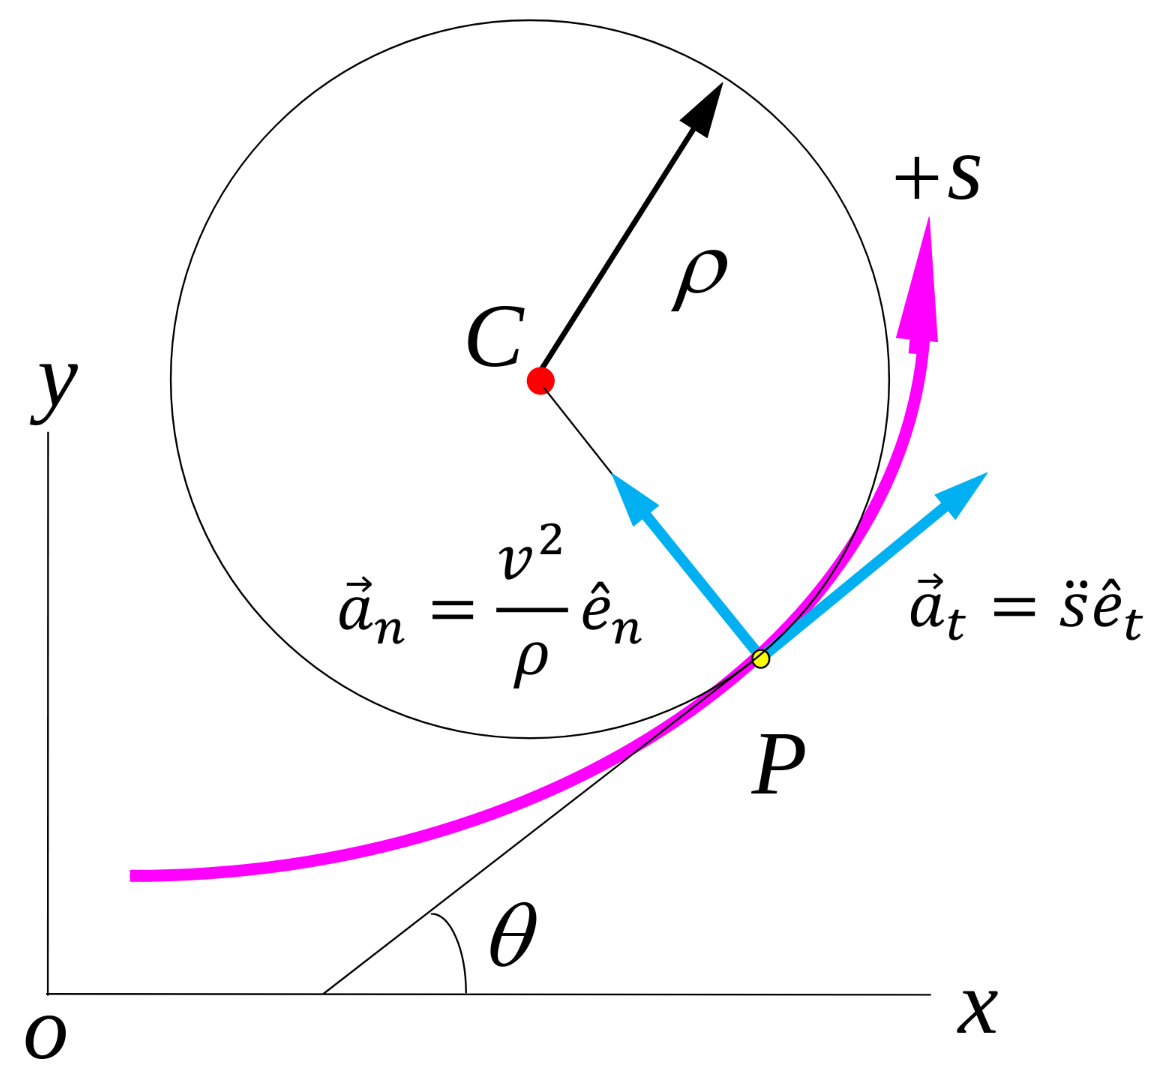
\includegraphics[scale=0.4]{./images/acceleration-in-path-coordinate-system.png}
\end{center}

\[\vec{a}_t = \ddot{s} \hat{e}_t\]
\[\vec{a}_n = \frac{v^2}{\rho} \hat{e}_n\]
\[\vec{a} = \vec{a}_t + \vec{a}_n\]

Where:
\begin{itemize}
\item \(\vec{a}_t\) is the tangential acceleration
\item \(\ddot{s}\) is the rate of change of the rate of change of the path coordinate
\item \(\hat{e}_t\) is the unit vector directed along the tangent to the path
\item \(\vec{a}_n\) is the normal or centripetal acceleration
\item \(v\) is the velocity of the particle
\item \(\rho\) is the radius of curvature of the path
\item \(\hat{e}_n\) is the unit vector directed towards the centre of curvature of the path
\item \(\vec{a}\) is the total acceleration
\end{itemize}

\subsection{Polar coordinate system}
\label{sec:org7be5210}
\begin{center}
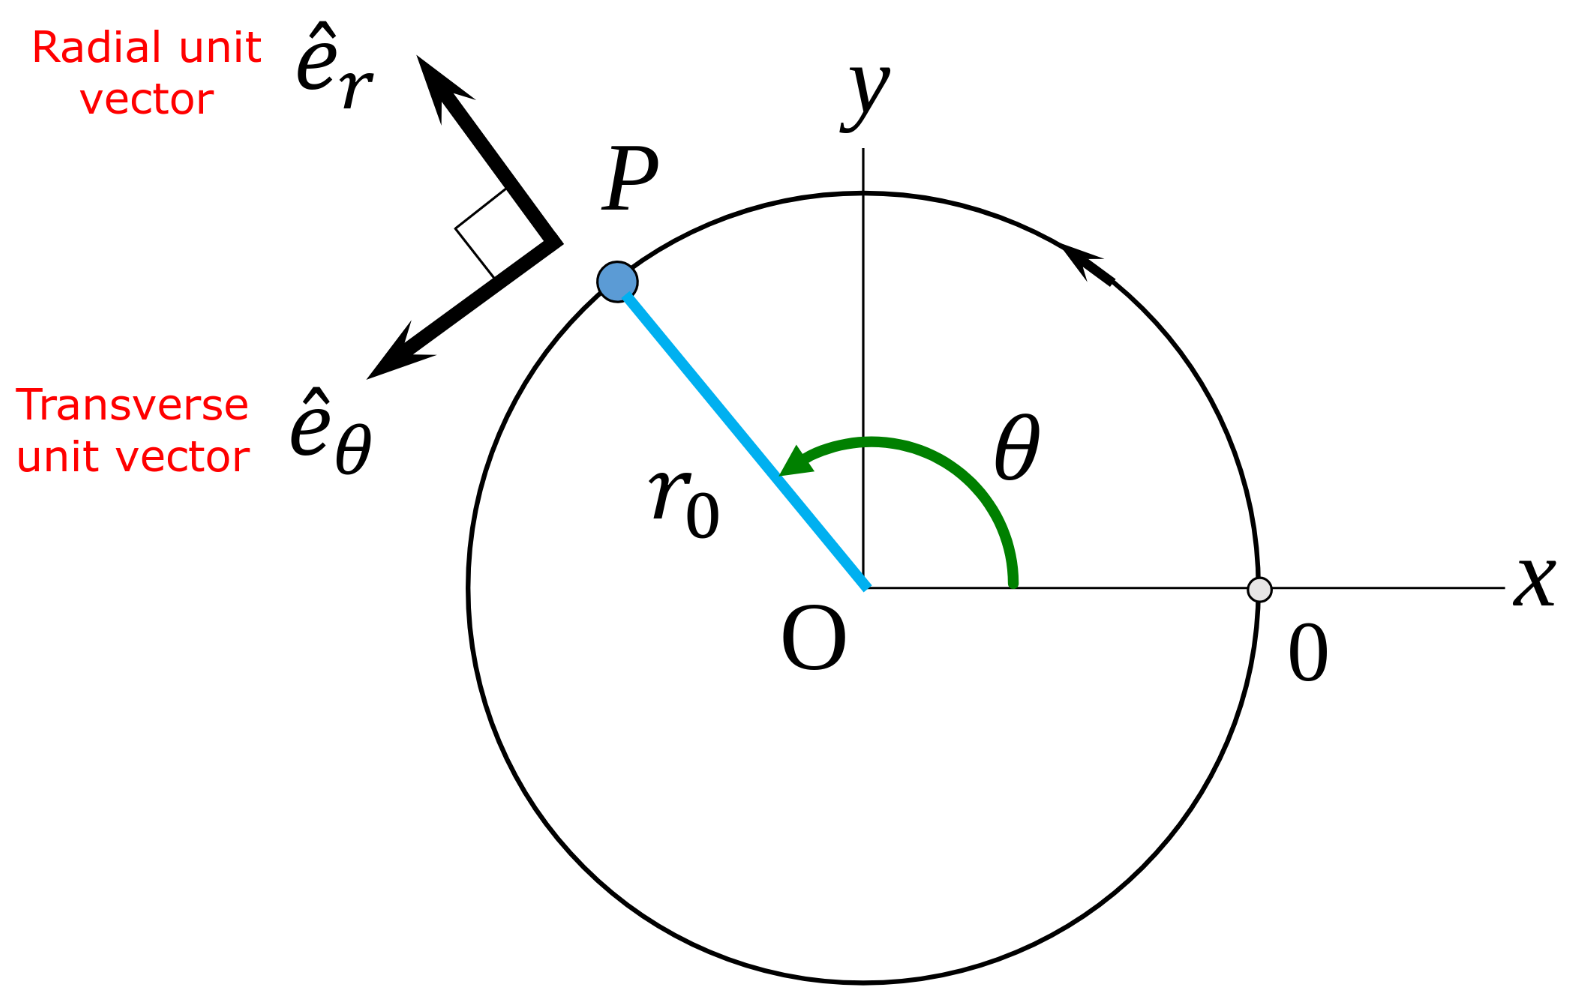
\includegraphics[width=.9\linewidth]{./images/polar-coordinates.png}
\end{center}
\[\theta = \frac{\text{Arc length}}{1}\]
\[\hat{e}_r = \cos \theta \hat{i} + \sin \theta \hat{j}\]
\[\hat{e}_{\theta} = - \sin \theta \hat{i} + \cos \theta \hat{j}\]
\[\vec{r} = r_0 \hat{e}_r = (r_0, \theta)\]

Where:
\begin{itemize}
\item \(\theta\) is the angle from the positive \(x\)-axis in the anti-clockwise direction
\item \(\hat{e}_r\) is the unit vector parallel to the position vector of the object
\item \(\hat{e}_{\theta}\) is the unit vector perpendicular to the position vector of the object, it is \(\hat{e}_r\) rotated \(90^{\circ}\) anti-clockwise
\item \(\vec{r}\) is the position vector of point \(P\)
\item \(r_0\) is the radius of the circle
\end{itemize}

\subsubsection{Kinematics equations}
\label{sec:org63a9dec}
\begin{center}
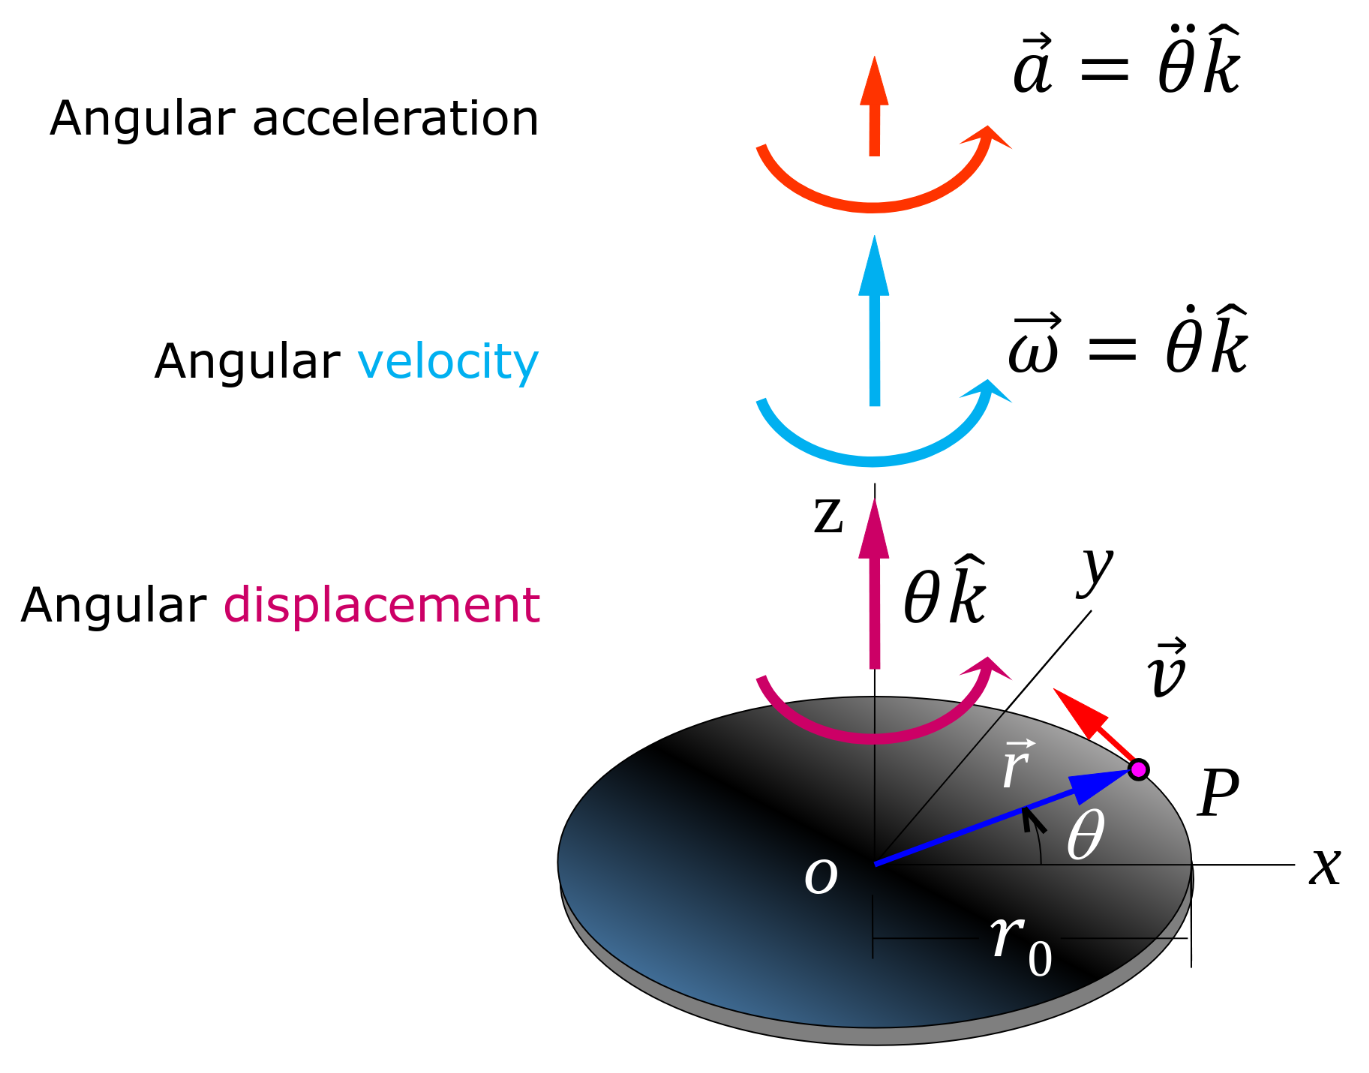
\includegraphics[width=.9\linewidth]{./images/polar-coordinates-kinematics-equations.png}
\end{center}
\[\text{Angular displacement} = \theta\]
\[\text{Angular velocity} = \frac{d}{dt} \theta = \dot{\theta}\]
\[\text{Angular acceleration} = \frac{d^2}{dt^2} \theta = \ddot{\theta}\]

\subsubsection{Polar coordinates vs Cartesian coordinates}
\label{sec:orge9b23db}
\begin{center}
\begin{tabular}{l|l}
Circular motion & Straight-line motion\\[0pt]
\hline
Polar coordinate (\(\hat{k}\)) & Cartesian coordinate (\(\hat{i}\))\\[0pt]
\(\theta\) & \(x\)\\[0pt]
\(\omega = \dot{\theta}\) & \(v = \dot{x}\)\\[0pt]
\(\alpha = \ddot{\theta}\) & \(a = \ddot{x}\)\\[0pt]
\(\theta \hat{k}, \omega \hat{k}, \alpha \hat{k}\) & \(x \hat{i}, v \hat{i}, a \hat{i}\)\\[0pt]
\end{tabular}
\end{center}

 \newpage

\subsubsection{Velocity (\(\vec{v}\))}
\label{sec:org27c8af0}
\[\vec{v} = \dot{r} \hat{e}_r + r \dot{\theta} \hat{e}_{\theta}\]

Where:
\begin{itemize}
\item \(\vec{v}\) is the velocity vector of the object in polar coordinates
\item \(\dot{r}\) is the rate of change of the magnitude of the position vector
\item \(\hat{e}_r\) is the unit vector parallel to the position vector of the object
\item \(r\) is the magnitude of the position vector of the object
\item \(\dot{\theta}\) is the rate of change of the angular displacement, or the angular velocity
\item \(\hat{e}_{\theta}\) is the unit vector perpendicular to the position vector of the object, it is \(\hat{e}_r\) rotated \(90^{\circ}\) anti-clockwise
\end{itemize}

\subsubsection{Acceleration (\(\vec{a}\))}
\label{sec:orgad9b352}
\label{org4f8ac63}
\[\vec{a} = \ddot{r} \hat{e}_r + r \ddot{\theta} \hat{e}_{\theta} - r \dot{\theta}^2 \hat{e}_r + 2 \dot{r} \dot{\theta} \hat{e}_{\theta}\]

Where:
\begin{itemize}
\item \(\vec{a}\) is the acceleration vector of the object in polar coordinates
\item \(\ddot{r}\) is the rate of change of the rate of change of the magnitude of the position vector, or the magnitude of the acceleration of the object
\item \(\hat{e}_r\) is the unit vector parallel to the position vector of the object
\item \(\ddot{\theta}\) is the rate of change of the rate of change of the angular displacement of the object, or the magnitude of the angular acceleration of the object
\item \(\hat{e}_{\theta}\) is the unit vector perpendicular to the position vector of the object, it is \(\hat{e}_r\) rotated \(90^{\circ}\) anti-clockwise
\item \(r\) is the magnitude of the position vector of the object
\item \(\dot{\theta}\) is the rate of change of the angular displacement, or the angular velocity
\item \(\dot{r}\) is the rate of change of the magnitude of the position vector
\end{itemize}

 \newpage

\subsection{Entrained quantity}
\label{sec:orgc7a3edc}
Entrained quantity is the quantity imparted into an object by another object that it is in contact with. This quantity is usually either velocity or acceleration, but could be other physical quantities as well. For example, a bead sliding down a rotating wire will have a sliding velocity, and a velocity imparted to it due to the rotation of the wire. This imparted velocity is called the entrained velocity.

\subsection{Entraining point}
\label{sec:org040c906}
Entraining point is the point of contact between two moving objects, such that an entrained quantity is created, which is a quantity from one object is imparted into the other object and vice versa.

\subsection{Relative quantity}
\label{sec:orgfb5469e}
Relative quantity is a quantity of one object, like \(A\), measured with respect to another object, like \(B\). The quantity is usually either velocity or acceleration. It is given by:
\[\vec{q}_{A/B} = \vec{q}_A - \vec{q}_B\]

Where:
\begin{itemize}
\item \(\vec{q}_{A/B}\) is the relative quantity of object \(A\) with respect to \(B\)
\item \(\vec{q}_A\) is the absolute quantity of object \(A\)
\item \(\vec{q}_B\) is the absolute quantity of object \(B\)
\end{itemize}

 \newpage

\subsection{Absolute velocity}
\label{sec:org3a12464}
Absolute velocity is the sum of the relative velocity and the entrained velocity.

\begin{center}
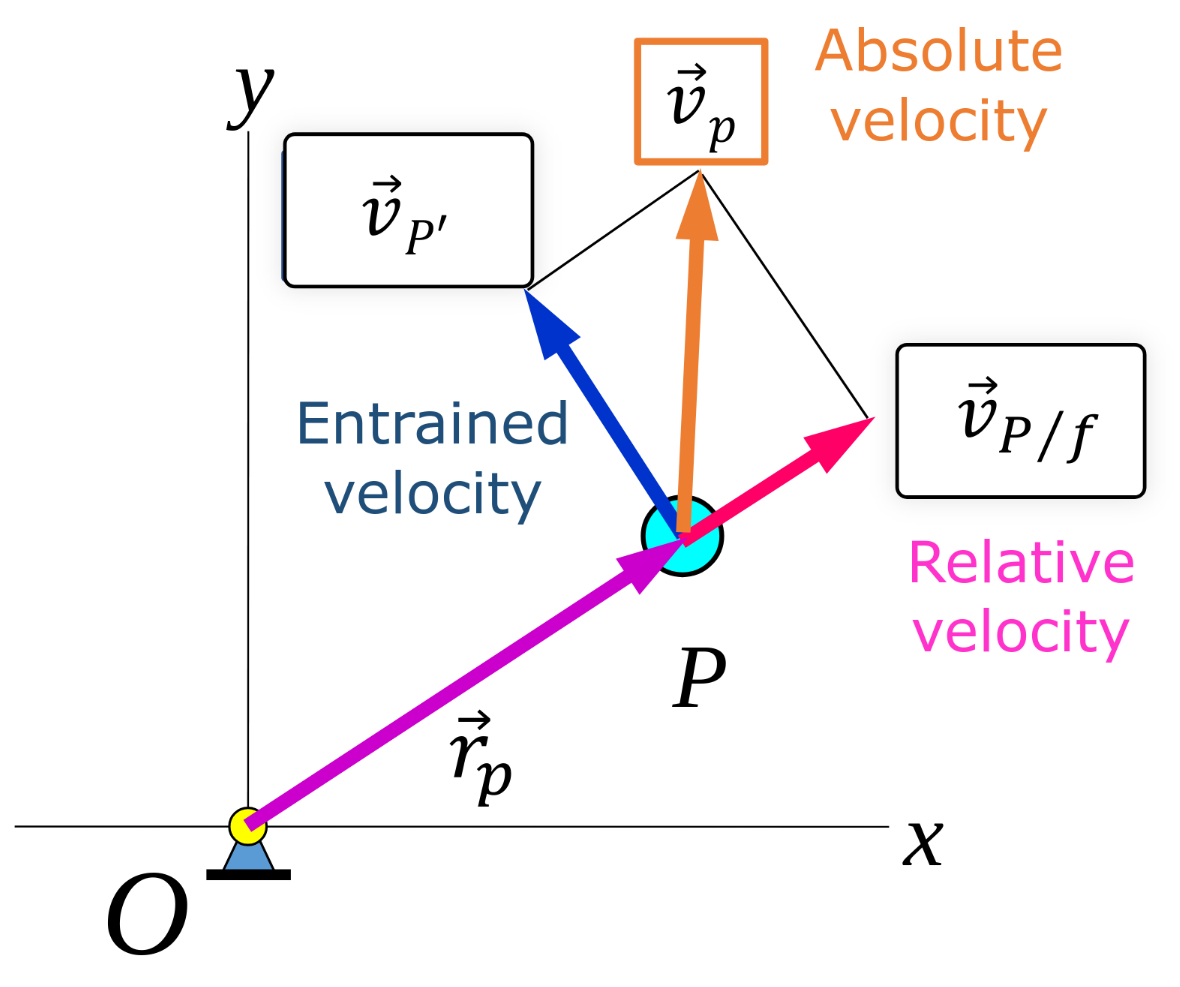
\includegraphics[width=.9\linewidth]{./images/different-types-of-velocities-in-curvilinear-motion.png}
\end{center}

\begin{center}
\begin{tabular}{c c c c c}
\(\vec{v}_p\) & \(=\) & \(\vec{v}_{p/f}\) & \(+\) & \(\vec{v}_{p'}\)\\[0pt]
Absolute velocity &  & Relative velocity &  & Entrained velocity\\[0pt]
 &  &  &  & \\[0pt]
Curvilinear & \(=\) & Rectilinear & \(+\) & Circular\\[0pt]
\end{tabular}
\end{center}

 \newpage

\subsection{Coriolis acceleration (\(\vec{a}_c\))}
\label{sec:org6728773}
\begin{itemize}
\item Coriolis acceleration is the acceleration experienced or observed by objects which are moving relative to a rotating frame of reference.
\item The Coriolis acceleration comes from 2 sources, and together they make up the total Coriolis acceleration, which is:
\end{itemize}

\[\vec{a}_c = 2 \dot{r} \dot{\theta} \hat{e}_{\theta}\]

Where:
\begin{itemize}
\item \(\vec{a}_c\) is the Coriolis acceleration
\item \(\dot{r}\) is the rate of change of position of the sliding object, which is the magnitude of the radial velocity
\item \(\hat{e}_r\) is the unit vector parallel to the position vector of the object
\item \(\dot{\theta}\) is the rate of change of angular displacement, or the angular velocity
\item \(\hat{e}_{\theta}\) is the unit vector perpendicular to the position vector of the object, it is \(\hat{e}_r\) rotated \(90^{\circ}\) anti-clockwise
\end{itemize}

 \newpage

\subsubsection{Change in radial velocity direction}
\label{sec:org9a68101}
\begin{center}
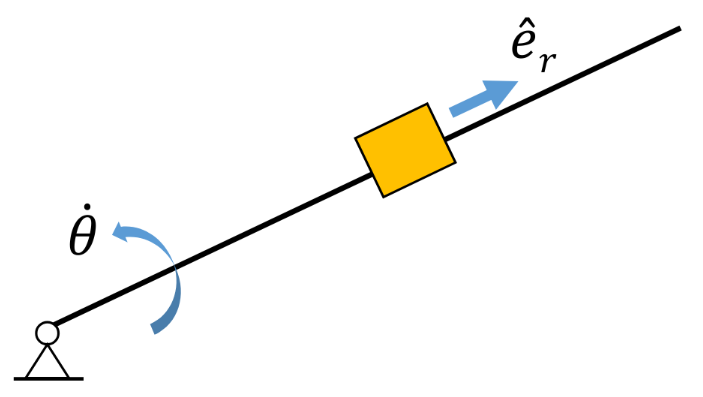
\includegraphics[width=.9\linewidth]{./images/change-in-radial-velocity-direction-coriolis-acceleration.png}
\end{center}
\begin{itemize}
\item The first source is due to the interaction of the radial velocity of the sliding object and the angular velocity imparted on the object.
\item While the magnitude of the radial velocity of the sliding object is constant, there is a change in the velocity's direction, which creates a tangential acceleration:
\end{itemize}

\[\vec{a}_t = \vec{\omega} \times \dot{r} \hat{e}_r = \dot{\theta} \dot{r} \hat{e}_{\theta}\]

Where:
\begin{itemize}
\item \(\vec{a}_t\) is the Coriolis acceleration that is tangential
\item \(\vec{\omega}\) is the angular velocity vector
\item \(\dot{r}\) is the rate of change of position of the sliding object, which is the magnitude of the radial velocity
\item \(\hat{e}_r\) is the unit vector parallel to the position vector of the object
\item \(\dot{\theta}\) is the rate of change of angular displacement, or the angular velocity
\item \(\hat{e}_{\theta}\) is the unit vector perpendicular to the position vector of the object, it is \(\hat{e}_r\) rotated \(90^{\circ}\) anti-clockwise
\end{itemize}

\subsubsection{Change in tangential velocity}
\label{sec:org07cde48}
\begin{center}
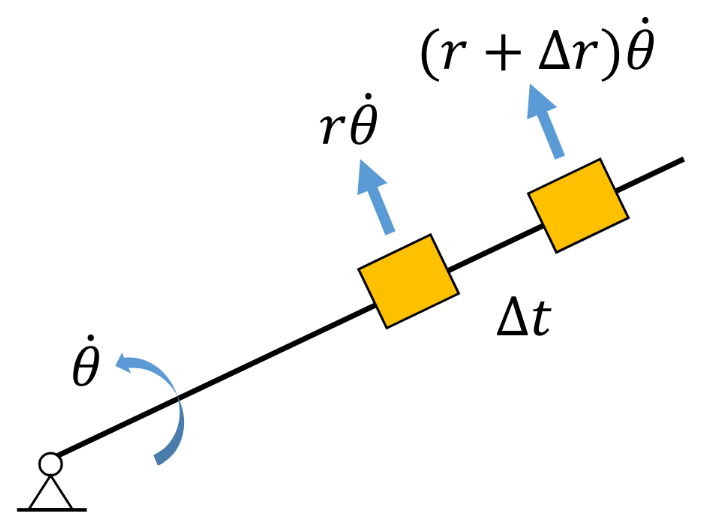
\includegraphics[scale=0.62]{./images/change-in-tangential-velocity-coriolis-acceleration.png}
\end{center}
\begin{itemize}
\item The second source is due to the change in tangential velocity of the sliding object.
\item The sliding object moves away from the centre of the circle it is rotating about.
\item This causes the distance of the object from the circle to increase from \(r\) to \(r + \Delta r\).
\item Since the object takes some time to move the distance \(\Delta r\), there is also a change in time \(\Delta t\).
\item This means that the tangential velocity has increased by \(\frac{\Delta r}{\Delta t} \dot{\theta}\), which also means there is an acceleration equal to \(\frac{\Delta r}{\Delta t} \dot{\theta}\).
\item Hence:
\end{itemize}

\[\vec{a}_t = \frac{\Delta r}{\Delta t} \dot{\theta} \hat{e}_{\theta} = \dot{r} \dot{\theta} \hat{e}_{\theta}\]

Where:
\begin{itemize}
\item \(\vec{a}_t\) is the Coriolis acceleration that is tangential
\item \(\Delta r\) is change in position of the object
\item \(\Delta t\) is the change in time
\item \(\dot{\theta}\) is the rate of change of angular displacement, or the angular velocity
\item \(\hat{e}_{\theta}\) is the unit vector perpendicular to the position vector of the object, it is \(\hat{e}_r\) rotated \(90^{\circ}\) anti-clockwise
\end{itemize}

\subsection{Absolute acceleration}
\label{sec:orgc705805}
\begin{center}
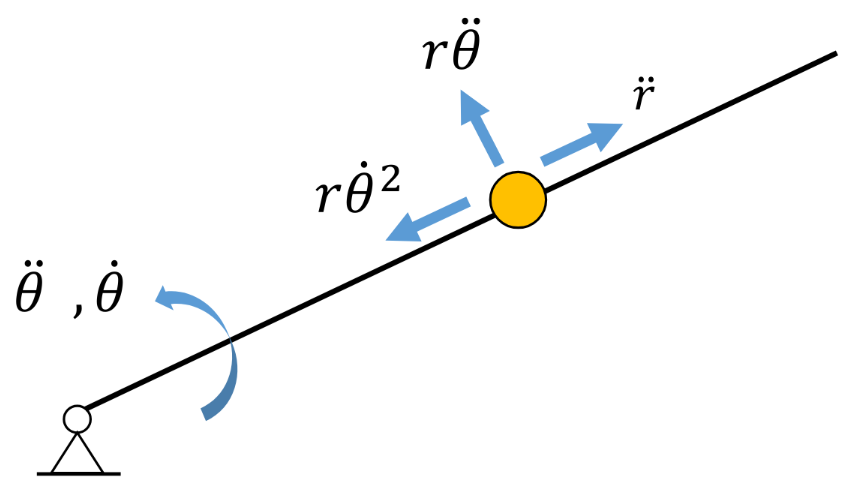
\includegraphics[width=.9\linewidth]{./images/absolute-acceleration-diagram.png}
\end{center}

\begin{center}
\begin{tabular}{>{\centering\arraybackslash}m{6em} >{\centering\arraybackslash}m{2em} >{\centering\arraybackslash}m{6em} >{\centering\arraybackslash}m{2em} >{\centering\arraybackslash}m{6em} >{\centering\arraybackslash}m{2em} >{\centering\arraybackslash}m{6em}}
\(\vec{a}_p\) & \(=\) & \(\vec{a}_{p/f}\) & \(+\) & \(\vec{a}_{p'}\) & \(+\) & \(\vec{a}_p^c\)\\[0pt]
Absolute acceleration &  & Relative acceleration &  & Entrained acceleration &  & Coriolis acceleration\\[0pt]
 &  &  &  &  &  & \\[0pt]
 &  & \(\ddot{r} \hat{e}_r\) & \(+\) & \((r \ddot{\theta} \hat{e}_{\theta} - r \dot{\theta}^2 \hat{e}_r)\) &  & \(2 \dot{r} \dot{\theta} \hat{e}_{\theta}\)\\[0pt]
\end{tabular}
\end{center}

 \newpage

\subsection{One-dimensional relative motion}
\label{sec:orgc126840}
\begin{center}
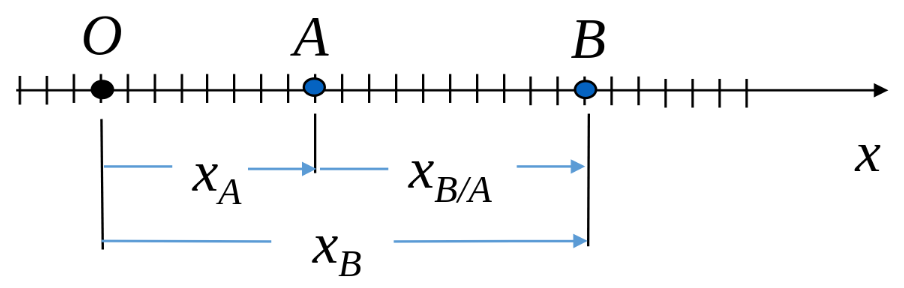
\includegraphics[width=.9\linewidth]{./images/one-dimensional-relative-motion.png}
\end{center}

When particles \(A\) and \(B\) move along the same straight line, the \textbf{relative motion} of \(B\) with respect to \(A\) can be considered. Denoting the relative position coordinate of \(B\) with respect to \(A\) as \(x_{B/A}\), we have:
\[x_B = x_A + x_{B/A}\]
\[v_B = v_A + v_{B/A}\]
\[a_B = a_A + a_{B/A}\]

Where:
\begin{itemize}
\item \(v_{B/A}\) is the relative velocity of B with respect to A
\item \(a_{B/A}\) is the relative acceleration of B with respect to A
\end{itemize}

 \newpage

\subsubsection{Pulley system}
\label{sec:orge44d5c3}
When several blocks are connected by \textbf{inextensible cords}, it is possible to write a linear relation between their position coordinates. Similar relations can then be written between their velocities and accelerations and can be used to analyse their motion.

\begin{center}
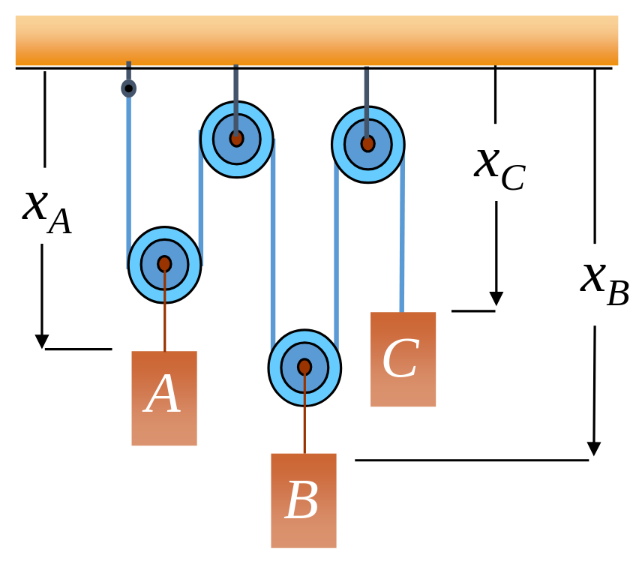
\includegraphics[width=.9\linewidth]{./images/pulley-system-diagram.png}
\end{center}

Steps to solving pulley system problems:
\begin{enumerate}
\item Define the position coordinates of all the blocks that move. The coordinates are determined relative to a fixed point, which is the origin.
\item Set up the constraint equations by expressing the length of the strings in the pulley system using the position coordinates of all the points of interests (the blocks that move).
\item Use the simultaneous equations to solve.
\item Differentiate the position coordinates with respect to time to find velocity and acceleration if necessary.
\end{enumerate}

\subsection{Two-dimensional relative motion}
\label{sec:org4df2248}
For two particles \(A\) and \(B\) moving in space, we consider the relative motion of \(B\) with respect to \(A\), or more precisely, with respect to a moving frame attached to \(A\) and in translation with \(A\). Denoting the relative position vector of \(B\) with respect to \(A\) as \(\vec{r}_B\), we have:
\[\vec{r}_B = \vec{r}_A + \vec{r}_{B/A}\]
\[\vec{v}_B = \vec{v}_A + \vec{v}_{B/A}\]
\[\vec{a}_B = \vec{a}_A + \vec{a}_{B/A}\]

Where:
\begin{itemize}
\item \(\vec{v}_{B/A}\) is the relative velocity of \(B\) with respect to \(A\)
\item \(\vec{a}_{B/A}\) is the relative acceleration of \(B\) with respect to \(A\)
\end{itemize}

\subsubsection{Relative velocity}
\label{sec:org3e3a47f}
The relative velocity with respect to \textbf{any fixed point} is the same.

\subsubsection{Relative acceleration}
\label{sec:org531c0a1}
The relative acceleration with respect to \textbf{any fixed point} is the same.

 \newpage

\subsection{Absolute velocity in circular motion}
\label{sec:orgda1879c}
\begin{center}
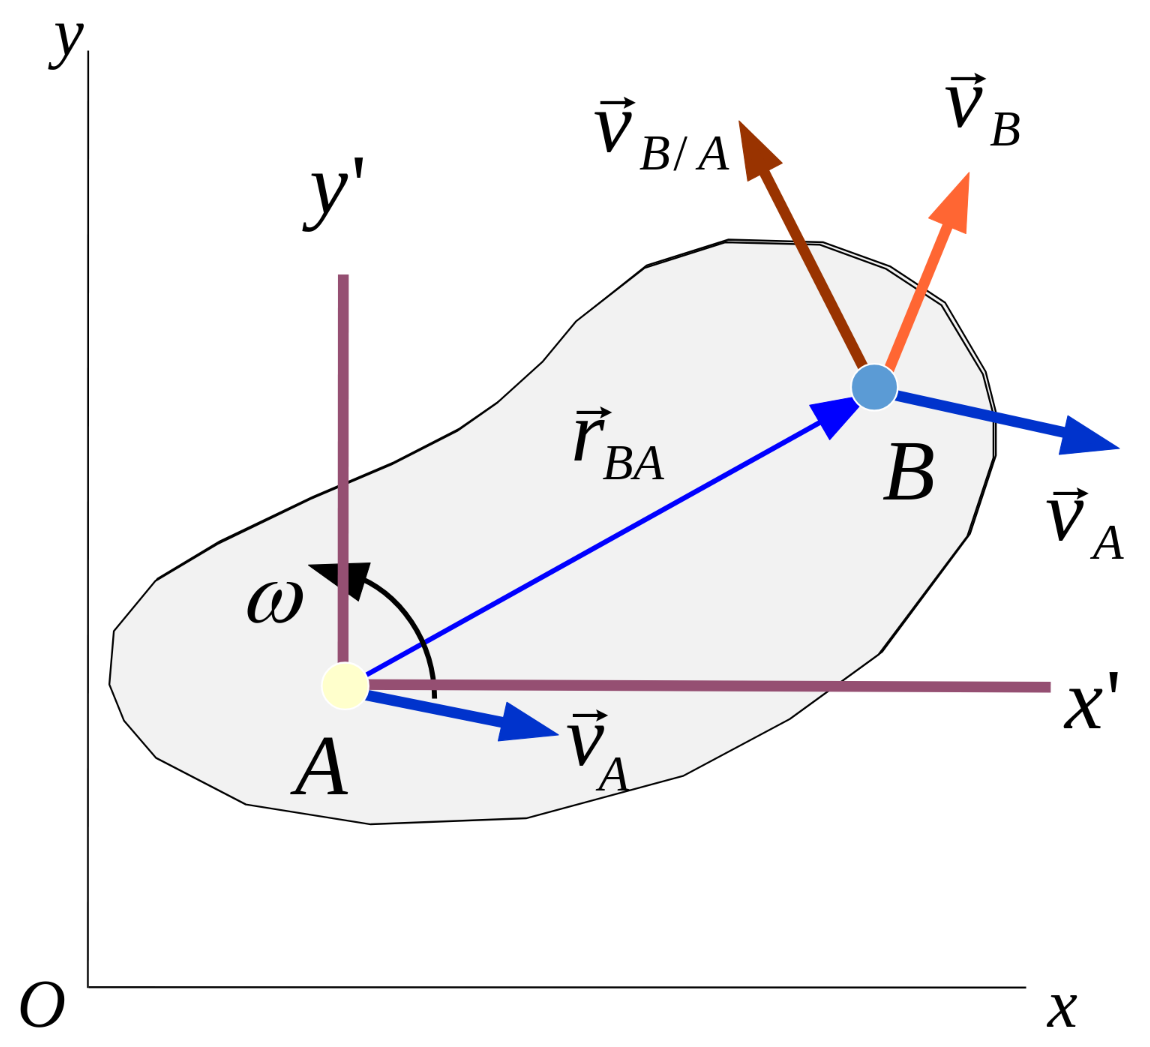
\includegraphics[scale=0.5]{./images/planar-motion-of-a-rigid-slab-velocity.png}
\end{center}

\begin{center}
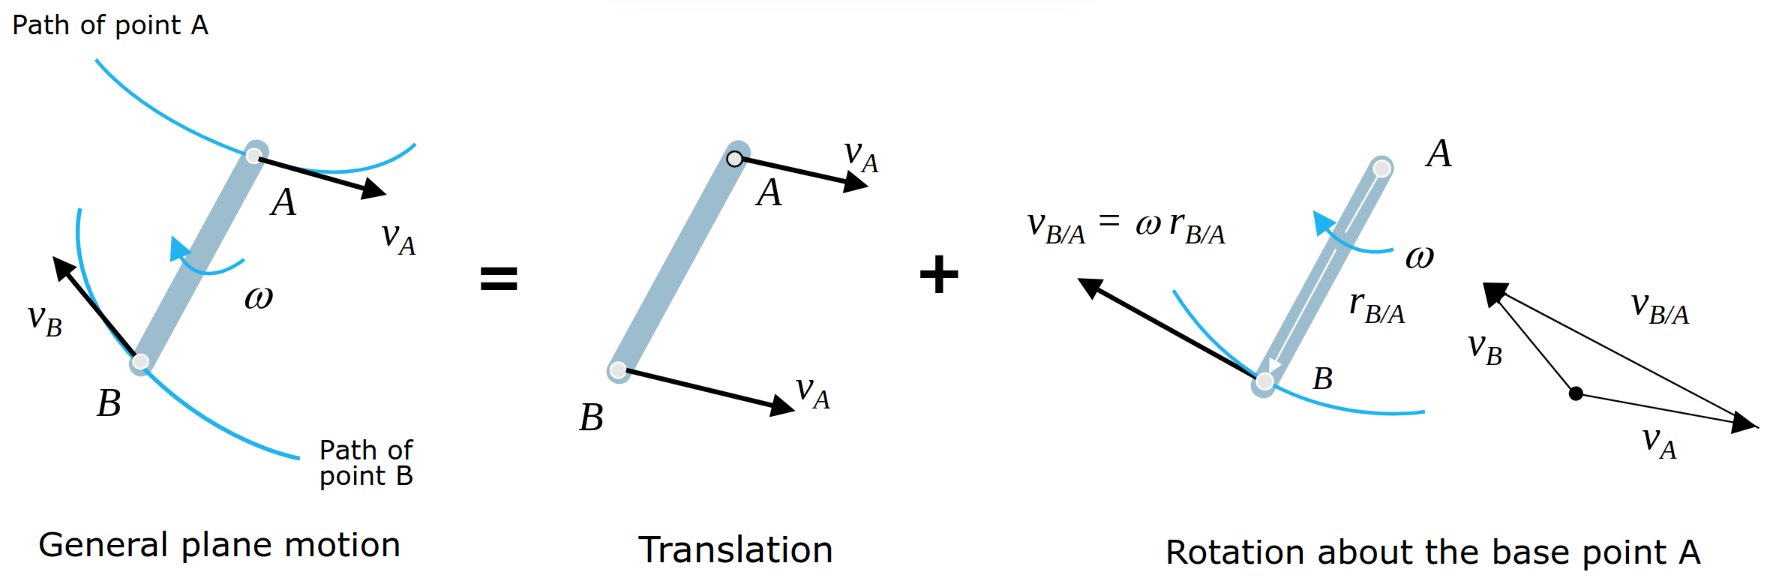
\includegraphics[width=.9\linewidth]{./images/relative-motion-analysis-velocity.png}
\end{center}
\[\vec{v}_B = \vec{v}_A + \vec{\omega} \times \vec{r}_{B/A}\]

\begin{itemize}
\item \(\vec{v}_B\) is determined by considering the entire body to translate with a velocity of \(\vec{v}_A\), and rotate about \(A\) with an angular velocity \(\vec{\omega}\)
\item Vector addition of these two effects, applied to \(B\), yields \(\vec{v}_B\)
\item \(\vec{v}_{B/A}\) represents the effect of circular motion about \(A\). It can be expressed by the cross product:
\[\vec{v}_{B/A} = \vec{\omega} \times \vec{r}_{B/A}\]
\end{itemize}

\subsection{Absolute acceleration in circular motion}
\label{sec:org1648ba4}
\begin{center}
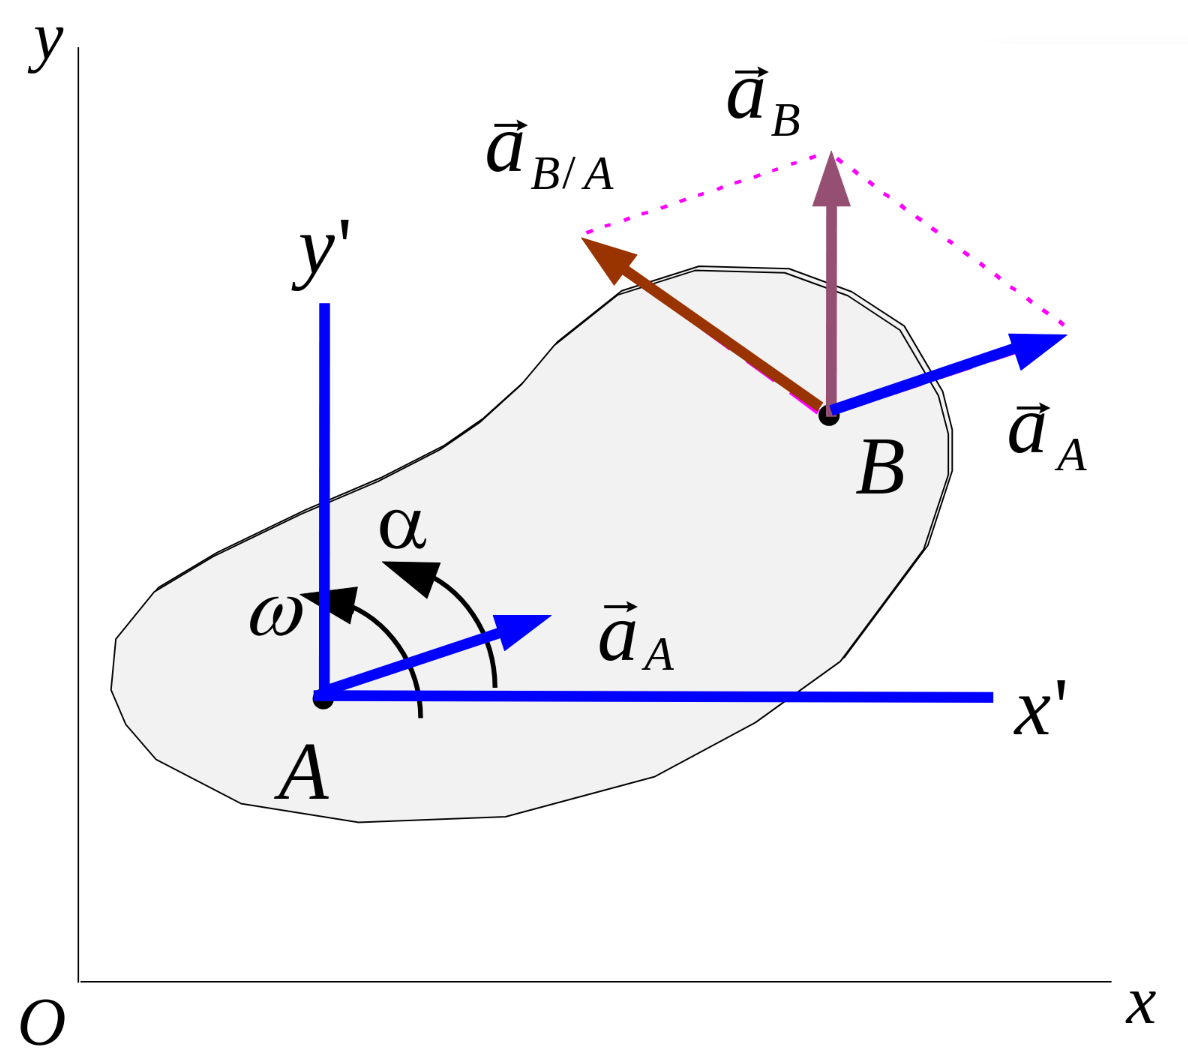
\includegraphics[width=.9\linewidth]{./images/planar-motion-of-a-rigid-slab-acceleration.png}
\end{center}
\begin{center}
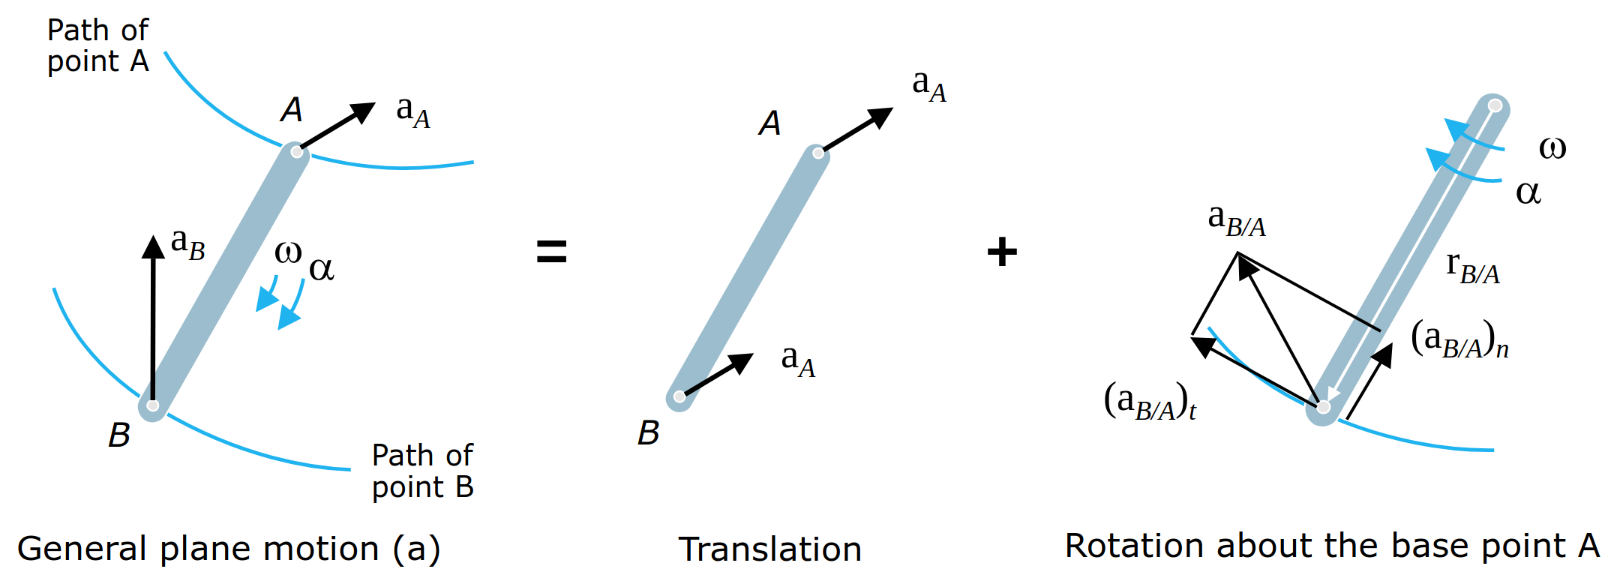
\includegraphics[width=.9\linewidth]{./images/relative-motion-analysis-acceleration.png}
\end{center}
\[\vec{a}_B = \vec{a}_A + \vec{\alpha} \times \vec{r}_{B/A} - \omega^2 \vec{r}_{B/A}\]

 \newpage

\subsection{Instantaneous centre of zero velocity (Instant centre)}
\label{sec:org3fa3d48}
\begin{itemize}
\item The instantaneous centre of zero velocity is a point that has zero velocity, at a \textbf{single instant in time}.
\item This instantaneous centre of zero velocity can be treated as a fixed point at which all points on the rigid object can be assumed to be in circular motion about.
\begin{center}
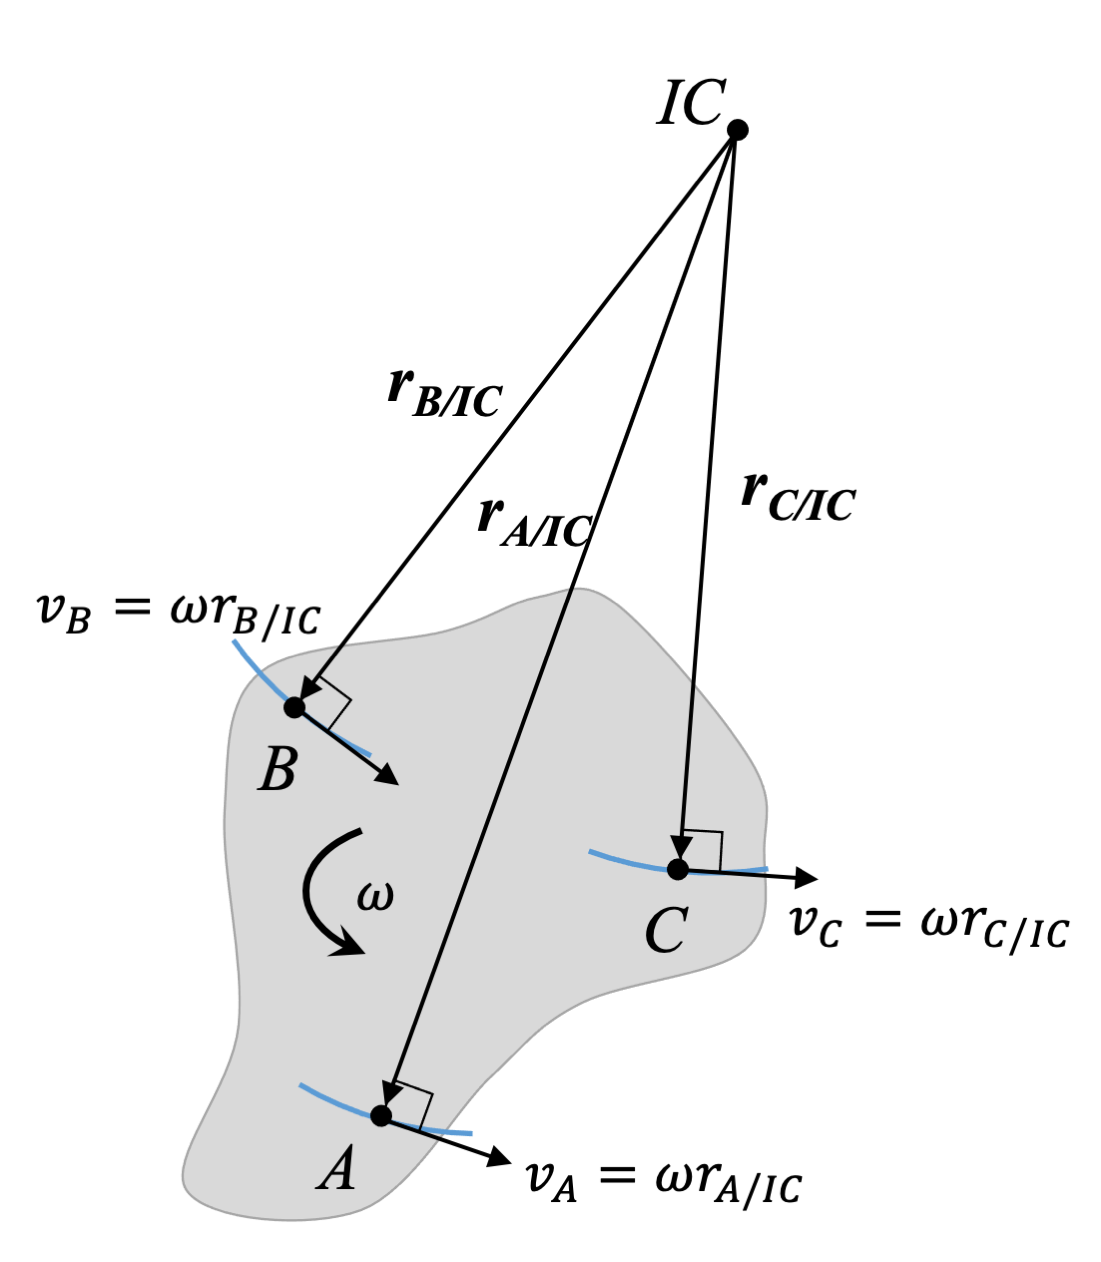
\includegraphics[width=.9\linewidth]{./images/instantaneous-centre-as-centre-of-rotation.png}
\end{center}
\end{itemize}

 \newpage

\subsubsection{Determining the instantaneous centre with non-parallel vectors}
\label{sec:org4b4be6c}
\begin{enumerate}
\item Get the direction of the 2 vectors.
\begin{center}
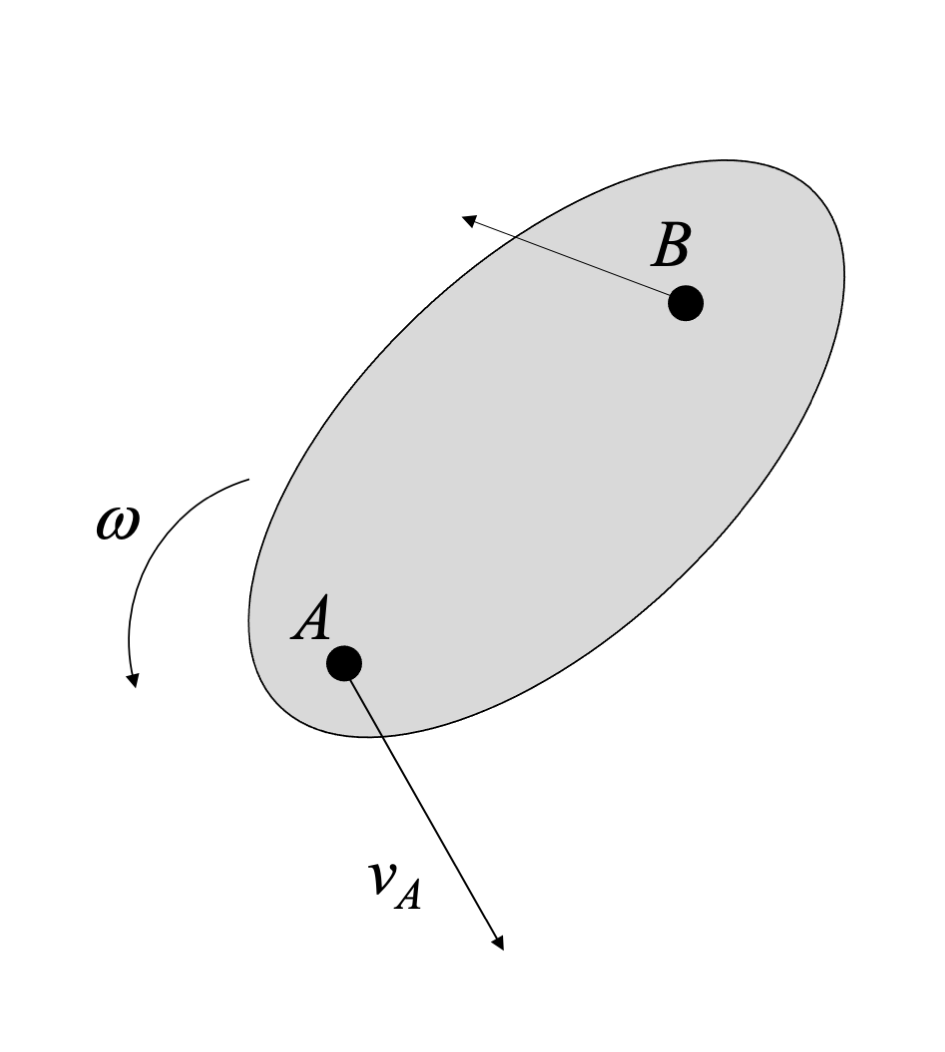
\includegraphics[scale=0.4]{./images/instantaneous-centre-non-parallel-vectors-first-step.png}
\end{center}
\item Draw a line perpendicular to each of the vectors.
\begin{center}
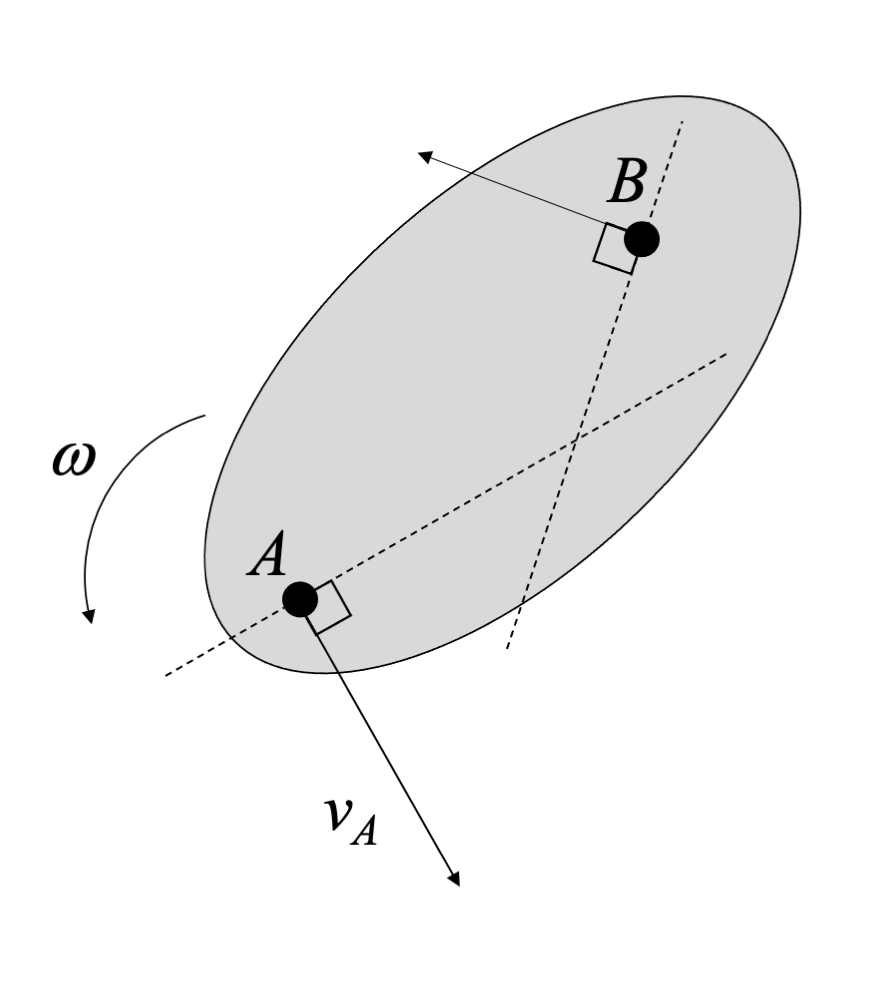
\includegraphics[scale=0.4]{./images/instantaneous-centre-non-parallel-vectors-second-step.png}
\end{center}
\item The intersection of the two lines is the instantaneous centre of zero velocity.
\end{enumerate}

 \newpage

\subsubsection{Determining the instantaneous centre with parallel vectors}
\label{sec:orgfba6639}
\begin{enumerate}
\item Draw a line that passes through the start of the 2 vectors.
\item Get the magnitude and direction of the 2 vectors.
\item Draw a line that connects the ends of the 2 vectors.
\item Depending on the direction and magnitude of the 2 vectors, there can be 3 cases as illustrated below.
\begin{center}
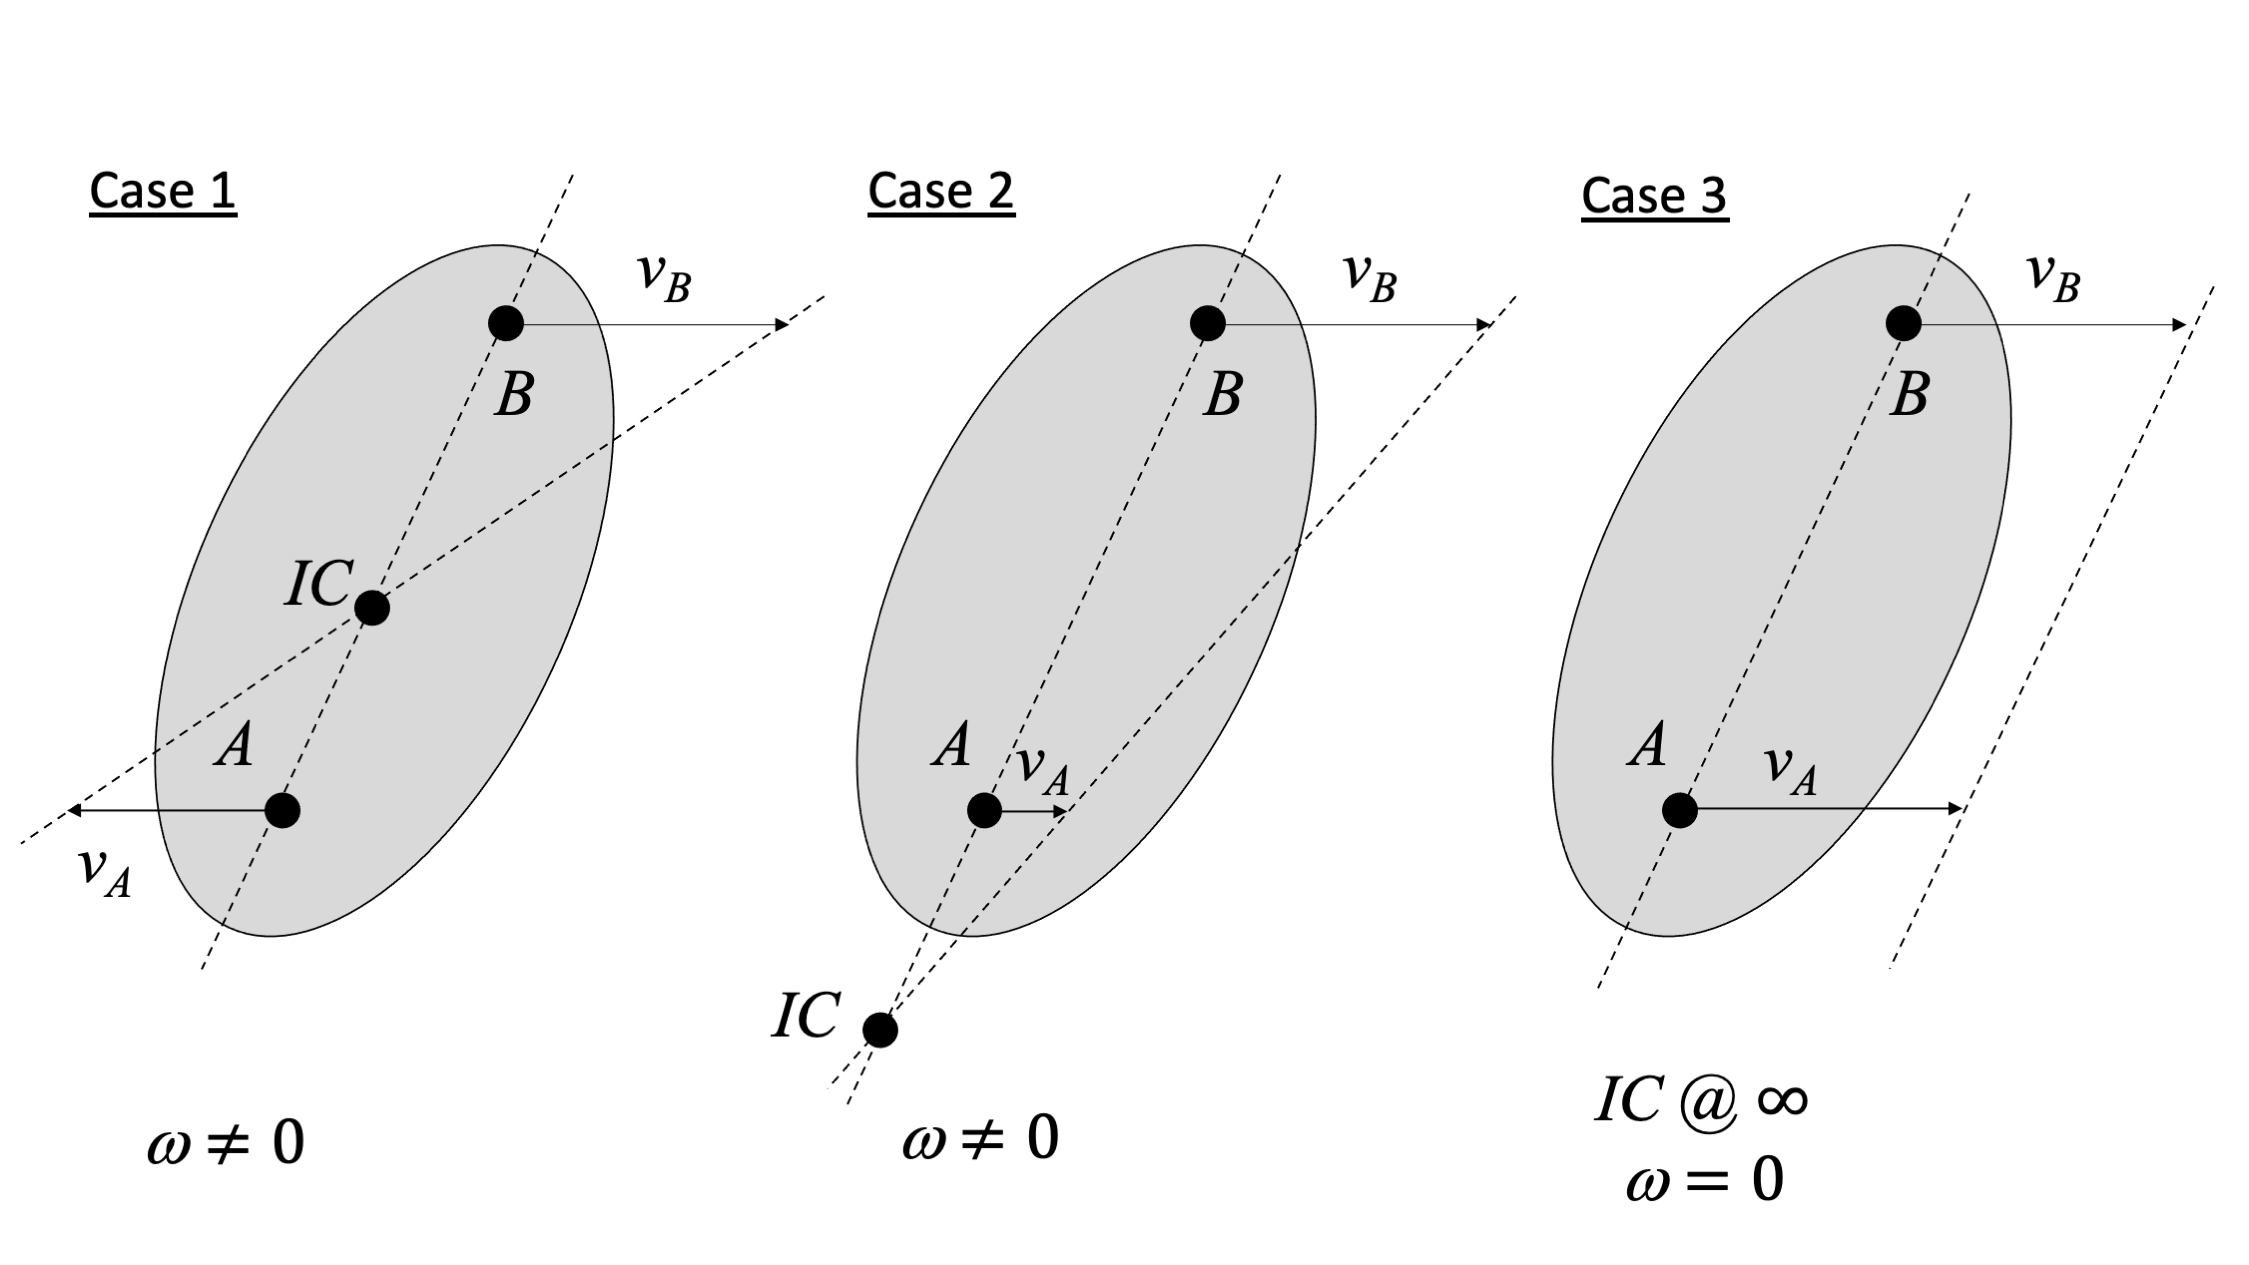
\includegraphics[width=.9\linewidth]{./images/instantaneous-centre-parallel-vectors.png}
\end{center}
\end{enumerate}

\subsection{Point of sliding contact with a body}
\label{sec:orgb72f550}
A point of sliding contact with a body must have a velocity that is tangential to the curvature of the body. This means that there cannot be a velocity component directed inwards or outwards from the body, or in two words, no penetration of the body by the velocity.

\begin{center}
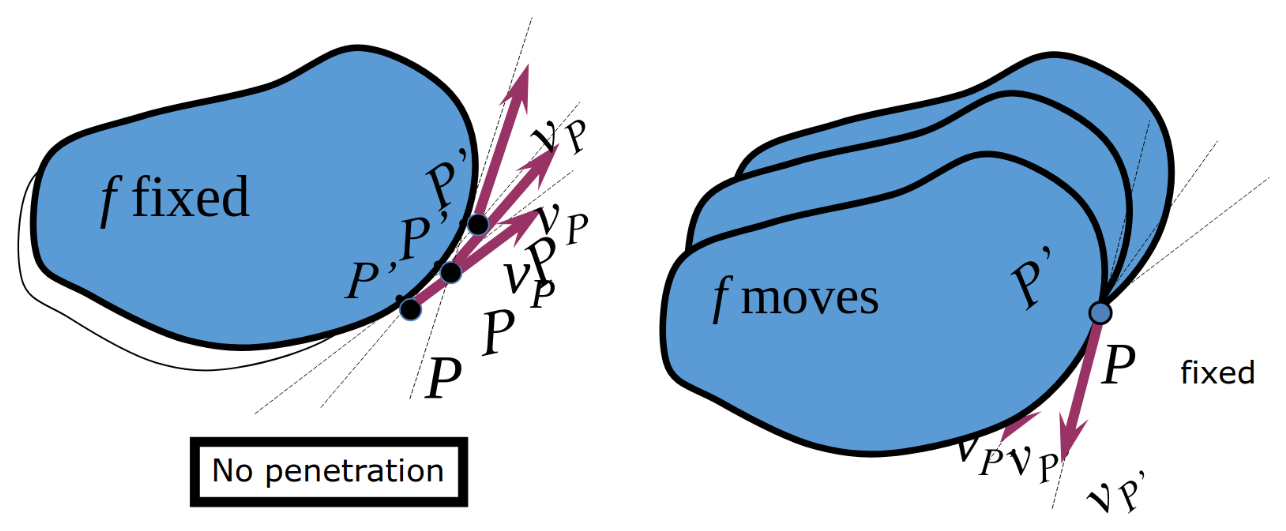
\includegraphics[width=.9\linewidth]{./images/sliding-contact-of-a-point.png}
\end{center}

\subsection{Velocity combination equation}
\label{sec:org58b2895}
\begin{center}
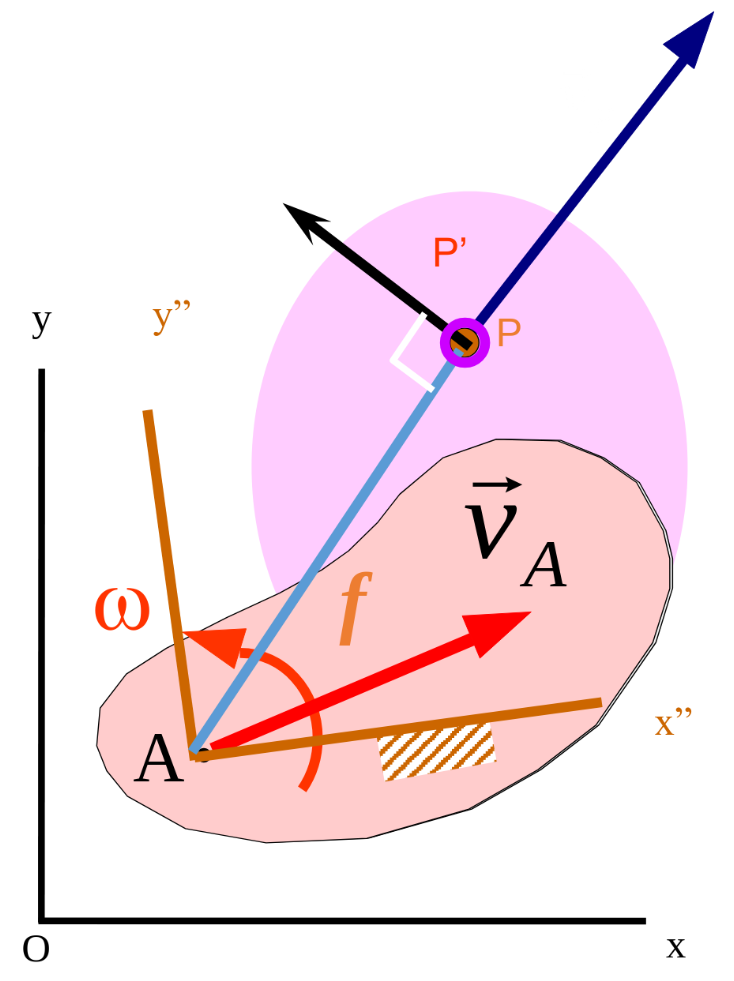
\includegraphics[height=30em]{./images/velocity-combination-equation-diagram.png}
\end{center}

\[\vec{v}_P = \vec{v}_{P/f} + \vec{v}_A + \vec{\omega}_f \times \vec{r}_{PA}\]

Where:
\begin{itemize}
\item \(\vec{v}_P\) is the absolute velocity of the point \(P\)
\item \(\vec{v}_{P/f}\) is the relative velocity of the point \(P\) with respect to the rotating and translating frame \(f\)
\item \(\vec{v}_A\) is the absolute velocity of the point \(A\) on the rotating and translating frame \(f\)
\item \(\vec{\omega}\) is the angular velocity of the rotating and translating frame \(f\)
\item \(\vec{r}_{PA}\) is the position vector of the point \(P\) with respect to the point \(A\)
\end{itemize}

\subsection{Acceleration combination equation}
\label{sec:org7ccd33c}
\begin{center}
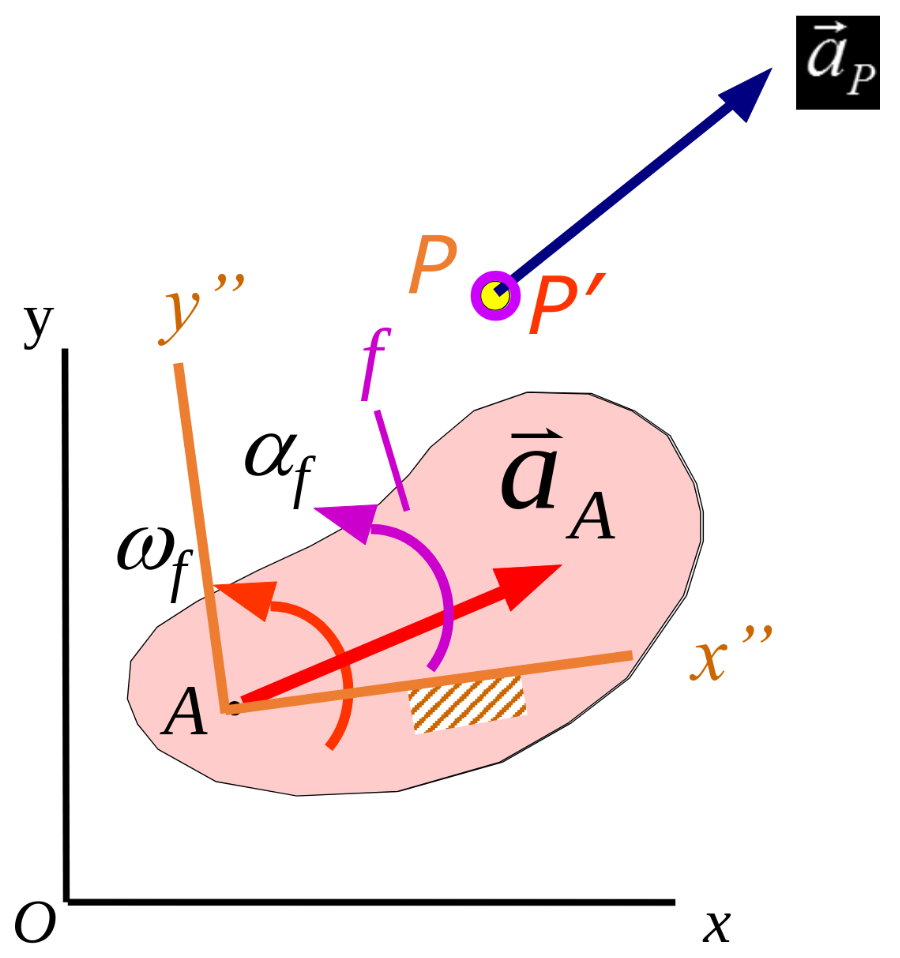
\includegraphics[height=29em]{./images/acceleration-combination-equation-diagram.png}
\end{center}

\[\vec{a}_P = \vec{a}_{P/f} + \vec{a}_{P'} + 2 \vec{\omega}_f \times \vec{v}_{P/f}\]

Where:
\begin{itemize}
\item \(\vec{a}_P\) is the absolute acceleration of the point \(P\)
\item \(\vec{a}_{P/f}\) is the relative acceleration of point \(P\) with respect to the rotating and translating frame \(f\)
\item \(\vec{a}_{P'}\) is entrained acceleration of the point \(P\), which is given by \(r \ddot{\theta} \hat{e}_{\theta} - r \dot{\theta}^2 \hat{e}_r\), the meaning of the symbols are given in this \hyperref[org4f8ac63]{section}.
\item \(\vec{\omega}_f\) is the angular velocity of the rotating and translating frame \(f\)
\item \(\vec{v}_{P/f}\) is the relative velocity of the point \(P\) with respect to the rotating and translating frame \(f\)
\end{itemize}

\subsection{Moment of inertia of a particle (\(I\))}
\label{sec:org8253f28}
\[I = mr^2\]

Where:
\begin{itemize}
\item \(I\) is the moment of inertia of the particle
\item \(m\) is the mass of the particle
\item \(r\) is the radius of the particle from the centre of the circle
\end{itemize}

\subsection{Momentum}
\label{sec:org4ea0fc3}

\subsubsection{Linear momentum (\(\vec{L}\))}
\label{sec:org44cf562}
\[\vec{L} = m \vec{v}\]

Where:
\begin{itemize}
\item \(\vec{L}\) is the linear momentum of the object
\item \(m\) is the mass of the object
\item \(\vec{v}\) is the velocity of the object
\end{itemize}

\subsubsection{Angular momentum (\(\vec{H}\))}
\label{sec:orga3b35fc}
\[\vec{H} = I \vec{\omega}\]

Where:
\begin{itemize}
\item \(\vec{H}\) is the angular momentum of the object
\item \(I\) is the moment of inertia of the object
\item \(\vec{\omega}\) is the angular velocity of the object
\end{itemize}

\subsection{Torque (\(\vec{M}\))}
\label{sec:org97182ae}
\[\vec{M} = \vec{r} \times \vec{F}\]

Where:
\begin{itemize}
\item \(\vec{M}\) is the torque acting on the object
\item \(\vec{r}\) is the perpendicular distance from the force to the pivot point on the object
\item \(\vec{F}\) is the force acting on the object
\end{itemize}

\subsubsection{Circular motion}
\label{sec:orge5c061c}
\[\vec{M} = I \vec{\alpha}\]

Where:
\begin{itemize}
\item \(\vec{M}\) is the torque acting on the object
\item \(I\) is the moment of inertia of the object
\item \(\vec{\alpha}\) is the angular acceleration of the object
\end{itemize}

\subsection{Newton's second law}
\label{sec:org379ff53}

\subsubsection{Acceleration form}
\label{sec:org951cc4a}
\[\vec{F} = m \vec{a}\]

Where:
\begin{itemize}
\item \(\vec{F}\) is the force acting on the object
\item \(m\) is the mass of the object
\item \(\vec{a}\) is the acceleration of the object
\end{itemize}

\subsubsection{Momentum form}
\label{sec:org0c572a2}
\[\vec{F} = \frac{d}{dt} \vec{L} = \frac{m \vec{v}}{\Delta t}\]

Where:
\begin{itemize}
\item \(\vec{F}\) is the force acting on the object
\item \(\frac{d}{dt} \vec{L}\) is the rate of change of linear momentum with respect to time
\item \(m\) is the mass of the object
\item \(v\) is the velocity of the object
\item \(\Delta t\) is the change in time
\end{itemize}

\subsubsection{Torque form}
\label{sec:org6a337e8}
\[\vec{r} \times \vec{F} = \frac{d}{dt} \left(\vec{r} \times \vec{L} \right)\]
\[\vec{M} = \frac{d}{dt} \vec{H}\]

Where:
\begin{itemize}
\item \(\vec{r}\) is the perpendicular distance from the force to the pivot point on the object
\item \(\vec{F}\) is the force acting on the object
\item \(\frac{d}{dt}\) is the rate of change with respect to time
\item \(\vec{L}\) is the linear momentum of the object
\item \(\vec{M}\) is the torque acting on the object
\item \(\frac{d}{dt} \vec{H}\) is the rate of change of angular momentum with respect to time
\end{itemize}

\subsection{Static friction (\(f_s\))}
\label{sec:orga6c111e}
Static friction varies, so it is not always \(f_s = \mu_s N\).
\(\mu_s N\) is just the maximum value of static friction.
\[-\mu_s N \le f_s \le \mu_s N\]

Where:
\begin{itemize}
\item \(f_s\) is the static friction
\item \(\mu_s\) is the coefficient of static friction
\item \(N\) is the normal contact force on the body
\end{itemize}

\subsection{Kinetic friction (\(f_k\))}
\label{sec:org2563b5e}
Kinetic friction is always constant.
\[f_k = \mu_k N\]

Where:
\begin{itemize}
\item \(f_k\) is the kinetic friction
\item \(\mu_s\) is the coefficient of kinetic friction
\item \(N\) is the normal contact force on the body
\end{itemize}

\subsection{Work done (\(U\))}
\label{sec:org420cf4b}
\[U = \int F \, dx\]
\[U = \int \vec{F} \cdot d \vec{r}\]

Where:
\begin{itemize}
\item \(U\) is the work done on the object
\item \(F\) is the force on the object
\item \(x\) is the displacement of the object
\item \(\vec{F}\) is the force vector on the object
\item \(\vec{r}\) is the displacement vector of the object
\end{itemize}

\subsubsection{Circular motion}
\label{sec:org35661ad}
\[U = \int M \, d \theta\]

Where:
\begin{itemize}
\item \(U\) is work done on the object
\item \(M\) is the torque on the object
\item \(\theta\) is the angular displacement of the object
\end{itemize}

 \newpage

\subsection{Power (\(P\))}
\label{sec:org7b582f2}
Power is the rate of work done.
\[P = \frac{U}{t}\]
\[P = \vec{F} \cdot \vec{v}\]
\[P = \vec{F} \cdot \frac{d \vec{r}}{dt}\]

Where:
\begin{itemize}
\item \(P\) is the power
\item \(U\) is the work done
\item \(t\) is the time taken
\item \(\vec{F}\) is the force vector on the object
\item \(\vec{v}\) is the velocity vector on the object
\item \(\vec{r}\) is the displacement vector of the object
\end{itemize}

\subsection{Kinetic energy}
\label{sec:orgff9ae6e}
\[U_k = \frac{1}{2} m \vec{v}^2\]

Where:
\begin{itemize}
\item \(U_k\) is the kinetic energy of the object
\item \(m\) is the mass of the object
\item \(\vec{v}\) is the velocity vector of the object
\end{itemize}

\subsubsection{Circular motion}
\label{sec:orgd89d82a}
\[U_k = \frac{1}{2} I \vec{\omega}^2\]

Where:
\begin{itemize}
\item \(U_k\) is the kinetic energy of the object
\item \(I\) is the moment of inertia of the object
\item \(\vec{\omega}\) is the angular velocity vector of the object
\end{itemize}

\subsection{Work and kinetic energy relation}
\label{sec:org4cefca5}
\[U = \frac{1}{2} m \vec{v}_2^2 - \frac{1}{2} m \vec{v}_1^2\]

Where:
\begin{itemize}
\item \(U\) is the work done on the object
\item \(m\) is the mass of the object
\item \(\vec{v}_2\) is the final velocity vector of the object
\item \(\vec{v}_1\) is the initial velocity vector of the object
\end{itemize}

\subsubsection{Circular motion}
\label{sec:org5296003}
\[U = \frac{1}{2} I \vec{\omega}_2^2 - \frac{1}{2} I \vec{\omega}_1^2\]

\begin{itemize}
\item \(U\) is the work done on the object
\item \(I\) is the moment of inertia of the object
\item \(\vec{\omega}_2\) is the final angular velocity vector of the object
\item \(\vec{\omega}_1\) is the initial angular velocity vector of the object
\end{itemize}

\subsection{Impulse}
\label{sec:org845f0cc}
\[\vec{I} = \int \vec{F} \, dt = m \vec{v}_2 - m \vec{v}_1\]

Where:
\begin{itemize}
\item \(\vec{I}\) is the impulse of the object
\item \(\vec{F}\) is the force on the object
\item \(m\) is the mass of the object
\item \(\vec{v}_2\) is the final velocity of the object
\item \(\vec{v}_1\) is the initial velocity of the object
\end{itemize}

\subsubsection{Circular motion}
\label{sec:org9c9649c}
\[\vec{I} = \int \vec{M} \, dt = \vec{H}_2 - \vec{H}_1\]

Where:
\begin{itemize}
\item \(\vec{I}\) is the angular impulse of the object
\item \(\vec{M}\) is the torque on the object
\item \(\vec{H}_2\) is the final angular momentum of the object
\item \(\vec{H}_1\) is the initial angular momentum of the object
\end{itemize}

\subsection{Potential energy}
\label{sec:org3ca4655}

\subsubsection{Gravitational potential energy (\(E_g\))}
\label{sec:orgc87603a}
\[E_g = mgh\]

Where:
\begin{itemize}
\item \(E_g\) is the gravitational potential energy of the object
\item \(m\) is the mass of the object
\item \(h\) is the height of the object above the ground
\end{itemize}

\subsubsection{Elastic potential energy (\(E_e\))}
\label{sec:orgd89f960}
\[E_e = \frac{1}{2} kx^2\]

Where:
\begin{itemize}
\item \(E_e\) is the elastic potential energy
\item \(k\) is the spring constant
\item \(x\) is the extension or contraction of the spring, measured from its natural length
\end{itemize}

\subsection{Conservation of energy}
\label{sec:org52000cf}
The conservation of energy states that the initial energy of a system is equal to the final energy of the system, as energy cannot be created or destroyed, i.e.
\[E_1 = E_2\]

Where:
\begin{itemize}
\item \(E_1\) is the initial energy of the system
\item \(E_2\) is the final energy of the system
\end{itemize}

\subsubsection{Conservation of kinetic energy}
\label{sec:org7375bb6}
\[\frac{1}{2} m_A v_{A0}^2 + \frac{1}{2} m_B \vec{v}_{B0}^2 = \frac{1}{2} m_A v_{A1}^2 + \frac{1}{2} m_B v_{B1}^2\]

Where:
\begin{itemize}
\item \(m_A\) is the mass of the first object \(A\)
\item \(v_{A0}\) is the \textbf{initial} speed of the first object \(A\)
\item \(m_B\) is the mass of the first object \(B\)
\item \(v_{B0}\) is the \textbf{initial} speed of the first object \(B\)
\item \(v_{A1}\) is the \textbf{final} speed of the first object \(A\)
\item \(v_{B1}\) is the \textbf{final} speed of the first object \(B\)
\end{itemize}

\subsection{Forces}
\label{sec:orgd6bc0f8}

\subsubsection{Gravitational force (\(F_g\))}
\label{sec:orgad51eb2}
\[F_g = mg\]

Where:
\begin{itemize}
\item \(F_g\) is the gravitational force
\item \(m\) is the mass of the object
\item \(g\) is the gravitational acceleration, \(\qty{9.81}{m.s^{-2}}\)
\end{itemize}

\subsubsection{Elastic spring force (\(F_s\))}
\label{sec:org155127a}
\[F_s = kx\]

Where:
\begin{itemize}
\item \(F_s\) is the elastic spring force
\item \(k\) is the spring constant
\item \(x\) is the extension or contraction of the spring, measured from its natural length
\end{itemize}

\subsection{Conservation of momentum}
\label{sec:org09e7a22}

\subsubsection{Linear momentum}
\label{sec:org74ec8c7}
\[m_A \vec{v}_{A2} + m_B \vec{v}_{B2} = m_A \vec{v}_{A1} + m_B \vec{v}_{B1}\]

Where:
\begin{itemize}
\item \(m_A\) is the mass of the first object \(A\)
\item \(\vec{v}_{A2}\) is the \textbf{final} velocity of the first object \(A\)
\item \(m_B\) is the mass of the first object \(B\)
\item \(\vec{v}_{B2}\) is the \textbf{final} velocity of the first object \(B\)
\item \(\vec{v}_{A1}\) is the \textbf{initial} velocity of the first object \(A\)
\item \(\vec{v}_{B1}\) is the \textbf{initial} velocity of the first object \(B\)
\end{itemize}

 \newpage

\subsubsection{Angular momentum}
\label{sec:org8d9ee9d}
\[r_1 mv_1 = r_2 m v_2\]
\[m r_1^2 \omega_1 = m r_2^2 \omega_2\]

Where:
\begin{itemize}
\item \(r_1\) is the \textbf{initial} radius of the object from the centre of the circle
\item \(m\) is the mass of the object
\item \(v_1\) is the \textbf{initial} velocity of the object
\item \(r_2\) is the \textbf{final} radius of the object from the centre of the circle
\item \(v_1\) is the \textbf{final} velocity of the object
\item \(\omega_1\) is the \textbf{initial} angular velocity of the object
\item \(\omega_2\) is the \textbf{final} angular velocity of the object
\end{itemize}

\subsection{Coefficient of restitution (\(e\))}
\label{sec:org4d99b49}
The coefficient of restitution the percentage of kinetic energy conserved in a collision

\subsubsection{Perfectly elastic collision (\(e = 1\))}
\label{sec:org605a412}
A perfectly elastic collision is when there is no energy lost and hence \(e = 1\).

\subsubsection{Elastic-plastic collision (\(0 < e < 1\))}
\label{sec:orged19985}
An elastic-plastic collision is when there is some energy lost and hence \(0 < e < 1\).

\subsubsection{Perfectly plastic collision (\(e = 0\))}
\label{sec:org62b34ab}
A perfectly plastic collision is when all energy is lost, and hence \(e = 0\). The objects stick together after the collision.

\subsection{Restitution equation}
\label{sec:org3947e0e}
The restitution equation is always in the direction of the impact force, or the \(\hat{e}_n\) direction.
\[(v_{A1}^n - v_{B1}^n) = - e(v_{A0}^n - v_{B0}^n)\]
\[(v_{A/B}^n)_1 = -e (v_{A/B}^n)_0\]

Where:
\begin{itemize}
\item \(v_{A1}\) is the \textbf{final} speed of the first object \(A\)
\item \(v_{B1}\) is the \textbf{final} speed of the first object \(B\)
\item \(e\) is the coefficient of restitution, where \(0 \le e \le 1\)
\item \(v_{A0}\) is the \textbf{initial} speed of the first object \(A\)
\item \(v_{B0}\) is the \textbf{initial} speed of the first object \(B\)
\item \((v_{A/B})_1\) is the \textbf{final} velocity of object \(A\) with respect to object \(B\)
\item \((v_{A/B})_0\) is the \textbf{initial} velocity of object \(A\) with respect to object \(B\)
\end{itemize}

\subsection{Rigid body}
\label{sec:orgf7c28ef}
A rigid body is an idealisation of a solid body in which deformation is neglected.

\subsubsection{Motion}
\label{sec:org7ae137f}
A rigid body has translation and rotation.

\subsubsection{Distribution of mass}
\label{sec:orgc39c4ac}
\begin{itemize}
\item Centre of mass, \(G\)
\item Moment of inertia, \(I_G\)
\end{itemize}

\subsection{Centre of mass}
\label{sec:org2b7c3cd}

\subsubsection{Discretely distributed mass (\(x_G\))}
\label{sec:orgbc6677f}
\[x_G = \frac{\sum_{i = 1}^n x_i m_i}{\sum_{i = 1}^n m_i}\]
\[\sum_{i = 1}^n \vec{x}_{iG} m_i = 0\]

Where:
\begin{itemize}
\item \(x_G\) is the position of the centre of mass
\item \(x_i\) is the position of particle \(i\)
\item \(m_i\) is the mass of particle \(i\)
\end{itemize}

\subsubsection{Continuously distributed mass (\(\vec{r}_G\))}
\label{sec:orgc38a55e}
\[\vec{r}_G = \frac{\int \vec{r} \, dm}{\int dm}\]
\[\int (\vec{r} - \vec{r}_G) \, dm = 0\]

Where:
\begin{itemize}
\item \(\vec{r}_G\) is the vector representing centre of mass of the object
\item \(\vec{r}\) is the position vector of the object
\item \(dm\) is the infinitesimal mass element of the object
\item \(\int dm\) is the mass of the object
\end{itemize}

\subsection{Linear momentum for a continuously distributed mass}
\label{sec:orgb16af0e}
\[\vec{L} = \int \dot{\vec{r}} \, dm = \vec{v} \, dm\]

Where:
\begin{itemize}
\item \(\vec{L}\) is the linear momentum of the body
\item \(\dot{\vec{r}}\) is the rate of change of position of the body
\item \(dm\) is the infinitesimal mass element of the object
\item \(\vec{v}\) is the velocity of the object
\end{itemize}

\subsection{Principle of linear momentum for rigid bodies}
\label{sec:orga22bbc5}
\[\vec{F} = \frac{d}{dt} \vec{L} = m \vec{a}_G\]

Where:
\begin{itemize}
\item \(\vec{F}\) is the resultant force on the body
\item \(\vec{L}\) is the linear momentum of the body
\item \(m\) is the total mass of the body
\item \(\vec{a}_G\) is the acceleration of the centre of mass
\end{itemize}

\subsection{Moment of inertia of an object (\(I_G\))}
\label{sec:orgfd5c31b}
\[I_G = \int r^2 \, dm\]
\[dm = p \, dx dy\]
\[I_G = \int (x^2 + y^2) \, \rho \, dx dy\]

Where:
\begin{itemize}
\item \(dm\) is the infinitesimal mass element of the object
\item \(dx\) is the length of the infinitesimal element of the object
\item \(dy\) is the width of the infinitesimal element of the object
\item \(r\) is the distance to the centre of mass of the object
\item \(\rho\) is the density of the object
\end{itemize}

\subsection{Parallel axis theorem}
\label{sec:org60285b4}
\[I_A = I_G + mr_{GA}^2\]

Where:
\begin{itemize}
\item \(I_A\) is the moment of inertia at point \(A\)
\item \(I_G\) is the moment of inertia of the object at point \(G\)
\item \(m\) is the mass of the object
\item \(r_{GA}\) is the distance between point \(G\) and point \(A\)
\end{itemize}

\subsection{Rotation of a rigid body about its mass centre \(G\)}
\label{sec:org31ae17b}
\[\vec{M}_G = \frac{d}{dt} \vec{H}_G = I_G \vec{\alpha}\]

Where:
\begin{itemize}
\item \(\vec{M}_G\) is the moment of the rigid body about its mass centre \(G\)
\item \(\vec{H}_G\) is the angular momentum of the rigid body about its mass centre \(G\)
\item \(I_G\) is the moment of inertia of the rigid body about its mass centre \(G\)
\item \(\vec{\alpha}\) is the angular acceleration of the rigid body
\end{itemize}

\subsection{General planar motion of a rigid body}
\label{sec:org910d15b}
\[\vec{M}_C = \frac{d}{dt} \vec{H}_C = \vec{r}_{GC} \times (m \vec{a}_G) + I_G \vec{\alpha}\]
\[\vec{H}_C = \vec{r}_{GC} \times (m \vec{v}_G) + I_{G} \vec{\omega}\]

Where:
\begin{itemize}
\item \(\vec{M}\) is the moment of the body about point \(C\)
\item \(\vec{H}_C\) is the angular momentum of the body about point \(C\)
\item \(\vec{r}_{GC}\) is the position vector of the centre of mass of the body (\(G\)) with respect to point \(C\)
\item \(m\) is the mass of the body
\item \(\vec{a}_G\) is the acceleration of the centre of mass of the body (\(G\))
\item \(I_G\) is the moment of inertia of the body about its centre of mass (\(G\))
\item \(\vec{\alpha}\) is the angular acceleration of the body
\item \(\vec{v}_G\) is the velocity of the centre of mass of the body (\(G\))
\item \(\vec{\omega}\) is the angular velocity of the body
\end{itemize}

\subsection{Motion of a rigid body about a fixed point}
\label{sec:orgbc4f1df}
\[\vec{M}_O = \frac{d}{dt} \vec{H}_O = I_O \vec{\alpha}\]
\[H_O = I_O \omega\]

Where:
\begin{itemize}
\item \(\vec{M}_O\) is the moment of the body about the fixed point \(O\)
\item \(\vec{H}_O\) is the angular momentum of the body about the fixed point \(O\)
\item \(I_O\) is the moment of inertia of the body about the fixed point \(O\)
\item \(\vec{\alpha}\) is the angular acceleration of the body
\item \(\vec{H}_O\) is the magnitude of the angular momentum of the body about the fixed point \(O\)
\item \(\omega\) is the magnitude of the angular velocity of the body
\end{itemize}

\subsection{Work done by a body}
\label{sec:orgbeb195b}
\[U_{1 \rightarrow 2} = \int_1^2 \vec{F} \cdot d \vec{r}_G + \int_{\theta_1}^{\theta_2} M_G \, d \theta\]

Where:
\begin{itemize}
\item \(U_{1 \rightarrow 2}\) is the work done by a body from state 1 to state 2
\item \(\vec{F}\) is the resultant force on the body
\item \(\vec{r}_G\) is the position of the centre of mass of the body (\(G\))
\item \(M_G\) is the magnitude of the moment about the centre of mass of the body (\(G\))
\item \(\theta\) is the angle of rotation of the body
\end{itemize}

 \newpage

\subsection{Kinetic energy of a body (\(U_k\))}
\label{sec:org48168fb}
\[U_k = \frac{1}{2} mv_G^2 + \frac{1}{2} I_G \omega^2 = \frac{1}{2} I_O \omega^2\]

Where:
\begin{itemize}
\item \(U_k\) is the kinetic energy of the body
\item \(m\) is the mass of the body
\item \(v_G\) is the velocity of the centre of mass of the body (\(G\))
\item \(I_G\) is the moment of inertia about the centre of mass of the body (\(G\))
\item \(\omega\) is the magnitude of the angular velocity of the body
\item \(I_O\) is the moment of inertia about an instantaneous centre of rotation or a fixed point
\end{itemize}

\subsection{Principle of linear impulse and momentum (translation)}
\label{sec:org9643de9}
\begin{align*}
\vec{I}_{1 \rightarrow 2} &= \int_{t1}^{t2} \vec{F} \, dt \\
&= \vec{L}_2 - \vec{L}_1 \\
&= m \vec{v}_{G2} - m \vec{v}_{G1}
\end{align*}

Where:
\begin{itemize}
\item \(\vec{I}_{1 \rightarrow 2}\) is the linear impulse of the object from time 1 \(t1\) to time 2 \(t2\)
\item \(\vec{F}\) is the net force on the object
\item \(dt\) is the infinitesimal change in time
\item \(\vec{L}_2\) is the linear momentum at time 2 (\(t2\))
\item \(\vec{L}_1\) is the linear momentum at time 1 (\(t1\))
\item \(m\) is the mass of the object
\item \(\vec{v}_{G2}\) is the velocity of the centre of mass of the object (\(G\)) at time 2 (\(t2\))
\item \(\vec{v}_{G1}\) is the velocity of the centre of mass of the object (\(G\)) at time 1 (\(t1\))
\end{itemize}

\subsection{Principle of angular impulse and momentum (rotation)}
\label{sec:orgf1fdc23}
\begin{align*}
I_{1 \rightarrow 2}^{(ang)} &= \int_{t1}^{t2} M_G \, dt \\
&= H_{G2} - H_{G1} \\
&= I_G \omega_2 - I_G \omega_1
\end{align*}

Where:
\begin{itemize}
\item \(I_{1 \rightarrow 2}^{(ang)}\) is the angular impulse of the object from time 1 \(t1\) to time 2 \(t2\)
\item \(M_G\) is the moment about the centre of mass of the object (\(G\))
\item \(dt\) is the infinitesimal change in time
\item \(\vec{H}_2\) is the angular momentum at time 2 (\(t2\))
\item \(\vec{H}_1\) is the angular momentum at time 1 (\(t1\))
\item \(I_G\) is the moment of inertia about the centre of mass of the object (\(G\))
\item \(\omega_{2}\) is the angular velocity of the object (\(G\)) at time 2 (\(t2\))
\item \(\omega_{1}\) is the angular velocity of the object (\(G\)) at time 1 (\(t1\))
\end{itemize}

 \newpage

\section{Formulas}
\label{sec:orgabe6bc1}

\subsection{Velocity (\(v\))}
\label{sec:orgc08aada}
\[v = \frac{dx}{dt}\]

Where:
\begin{itemize}
\item \(v\) is the velocity of the particle
\item \(\frac{dx}{dt}\) is the derivative of the position of the particle with respect to time
\end{itemize}

\subsection{Acceleration (\(a\))}
\label{sec:org4dc9662}
\[a = \frac{dv}{dt}\]
\[a = \frac{d^2x}{dt^2}\]
\[a = v \frac{dv}{dx}\]

Where:
\begin{itemize}
\item \(a\) is the acceleration of the particle
\item \(\frac{dv}{dt}\) is the derivative of the velocity of the particle with respect to time
\item \(\frac{d^2x}{dt^2}\) is the second derivative of the position of the particle with respect to time
\item \(v\) is the velocity of the particle
\item \(\frac{dv}{dx}\) is the derivative of the velocity of the particle with respect to its position
\end{itemize}

 \newpage

\subsection{Circular motion}
\label{sec:org7068071}

\subsubsection{Angular displacement (\(\theta\))}
\label{sec:orgd750d97}
\[\theta = \frac{\text{Arc length}}{r}\]

Where:
\begin{itemize}
\item \(\theta\) is the angular displacement of the object in circular motion
\item \(r\) is the distance of the object from the centre of the circle
\end{itemize}

\subsubsection{Angular velocity (\(\vec{\omega}\))}
\label{sec:org31a36ac}
\[\vec{\omega} = \frac{2 \pi}{T} \hat{e}\]
\[\vec{\omega} = \frac{\theta}{t} \hat{e}\]
\[\vec{\omega} = \frac{\vec{v}}{r}\]

Where:
\begin{itemize}
\item \(\vec{\omega}\) is the angular velocity vector of the object in circular motion
\item \(T\) is the period
\item \(\theta\) is the angle rotated by the object in circular motion
\item \(t\) is the time taken for the object to rotate the angle \(\theta\)
\item \(\hat{e}\) is the direction vector perpendicular to the plane that the motion is taking place, usually \(\vec{k}\). Use the right-hand grip (screw) rule to figure out the direction of the angular velocity.
\item \(\vec{v}\) is the velocity vector of the object in circular motion
\item \(r\) is the distance of the object from the centre of the circle
\end{itemize}

 \newpage

\subsubsection{Angular acceleration (\(\vec{\alpha}\))}
\label{sec:orgcc6dfe0}
\[\vec{\alpha} = \frac{a_t}{r} \hat{e}\]
\[\vec{\alpha} = \frac{\vec{\omega}}{t}\]

Where:
\begin{itemize}
\item \(\vec{\alpha}\) is the angular acceleration of the object in circular motion
\item \(a_t\) is the magnitude of the tangential acceleration of the object in circular motion
\item \(\hat{e}\) is the direction vector perpendicular to the plane that the motion is taking place, usually \(\vec{k}\). Use the right-hand grip (screw) rule to figure out the direction of the angular velocity.
\item \(r\) is the distance of the object from the centre of the circle
\item \(\vec{\omega}\) is the angular velocity of the object in circular motion
\item \(t\) is the time taken for the object to rotate
\end{itemize}

\subsubsection{Position (\(\vec{r}\))}
\label{sec:orgb64054d}
\[\vec{r} = r_0 \vec{e}_r = r_0 (\cos \theta \hat{i} + \sin \theta \hat{j})\]

Where:
\begin{itemize}
\item \(\vec{r}\) is the position vector of an object in circular motion
\item \(r_0\) is the distance of the object away from the centre of the circle
\item \(\theta\) is the angular displacement
\end{itemize}

 \newpage

\subsubsection{Velocity (\(\vec{v}\))}
\label{sec:org8500c81}
\[\vec{v} = \frac{d \vec{r}}{dt} = \frac{d}{dt} (r_0 \hat{e}_r) = r_0 \frac{d \hat{e}_r}{dt}\]
\[\frac{d \hat{e}_r}{dt} = \dot{\theta} (- \sin \theta \hat{i} + \cos \theta \hat{j}) = \omega \hat{e}_{\theta}\]
\[\vec{v} = \vec{\omega} \times \vec{r}\]

Where:
\begin{itemize}
\item \(\vec{v}\) is the velocity vector of the object in circular motion
\item \(r_0\) is the distance of the object from the centre of the circle
\item \(\hat{e}_r\) is the unit vector parallel to the position vector of the object
\item \(\dot{\theta}\) is the rate of change of angular displacement
\item \(\theta\) is the angular displacement
\item \(\hat{e}_{\theta}\) is the unit vector perpendicular to the position vector of the object, it is \(\hat{e}_r\) rotated \(90^{\circ}\) anti-clockwise
\item \(\vec{\omega}\) is the angular velocity vector of the object
\item \(\vec{r}\) is the position vector of the object with respect to the centre of the circle, i.e. the centre of the circle is the origin
\end{itemize}

\subsubsection{Tangential acceleration (\(\vec{a}_t\))}
\label{sec:orgb440e9c}
\[\vec{a}_t = \vec{\alpha} \times \vec{r}\]

Where:
\begin{itemize}
\item \(\vec{a}\) is the tangential acceleration vector of the object in circular motion
\item \(\vec{\alpha}\) is the angular acceleration vector of the object
\item \(\vec{r}\) is the position vector of the object with respect to the centre of the circle, i.e. the centre of the circle is the origin
\end{itemize}

 \newpage

\subsubsection{Centripetal or normal acceleration (\(\vec{a}_n\))}
\label{sec:orgfba6892}
\[\vec{a}_n = \vec{\omega} \times \vec{v} = - \omega^2 \vec{r} = - \frac{v^2}{r} \hat{e}_{\theta}\]

Where:
\begin{itemize}
\item \(\vec{a}_n\) is the centripetal or normal acceleration of the object in circular motion
\item \(\vec{\omega}\) is the angular velocity vector of an object in circular motion
\item \(\vec{v}\) is the velocity vector of the object in circular motion
\item \(\omega\) is the magnitude of the angular velocity of an object in circular motion
\item \(\vec{r}\) is the position vector of the object with respect to the centre of the circle, i.e. the centre of the circle is the origin
\item \(v\) is the magnitude of the velocity vector
\item \(\hat{e}_{\theta}\) is the unit vector perpendicular to the position vector of the object, it is \(\hat{e}_r\) rotated \(90^{\circ}\) anti-clockwise
\end{itemize}

\subsubsection{Total acceleration (\(\vec{a}\))}
\label{sec:org1f4f7fb}
\[\vec{a} = \vec{a}_t + \vec{a}_n\]

Where:
\begin{itemize}
\item \(\vec{a}\) is the total acceleration of the object in circular motion
\item \(\vec{a}_t\) is the tangential acceleration of the object in circular motion
\item \(\vec{a}_n\) is the centripetal or normal acceleration of the object in circular motion
\end{itemize}

\subsection{Uniform rectilinear motion}
\label{sec:org26db264}
\[x = x_0 + vt\]

Where:
\begin{itemize}
\item \(x\) is the final position of the particle
\item \(x_0\) is the initial position of the particle
\item \(v\) is the velocity of the particle
\item \(t\) is the time taken by the particle
\end{itemize}

\subsection{Uniformly accelerated rectilinear motion}
\label{sec:org6763349}
\[v = v_0 + at\]
\[x = x_0 + v_0t + \frac{1}{2}at^2\]
\[v^2 = v_0^2 + 2a(x - x_0)\]

Where:
\begin{itemize}
\item \(v\) is the final velocity of the particle
\item \(x\) is the final position of the particle
\item \(a\) is the acceleration of the particle
\item \(t\) is the time take by the particle
\item \(v_0\) is the initial velocity of the particle
\item \(x_0\) is the initial position of the particle
\end{itemize}

\subsection{Velocity of a particle in curvilinear motion}
\label{sec:org5a7c2ee}
\[\vec{v} = \frac{d \vec{r}}{dt}\]
\[v = \frac{ds}{dt}\]

Where:
\begin{itemize}
\item \(\vec{v}\) is the velocity vector of the particle
\item \(\vec{r}\) is the current position vector of the particle from the origin \(O\)
\item \(dt\) is the infinitesimal change in time
\item \(v\) is the magnitude of the velocity vector
\item \(s\) is the arc length of particle, measured from the initial position of the particle
\end{itemize}

\subsection{Instantaneous velocity of a particle in curvilinear motion (\(\vec{v}_{instant}\))}
\label{sec:org03b99e1}
\[\vec{v}_{instant} \equiv \lim_{\Delta t \rightarrow 0} \frac{\Delta \vec{r}}{\Delta t} = \frac{d \vec{r}}{dt}\]

Where:
\begin{itemize}
\item \(\vec{v}_{instant}\) is the instantaneous velocity of the particle in curvilinear motion
\item \(\delta \vec{r}\) is the change in position vector of the particle
\item \(\delta t\) is the change in time
\item \(d \vec{r}\) is the change in position vector of the particle
\item \(dt\) is the infinitesimal change in time
\end{itemize}

\subsection{Acceleration of a particle in curvilinear motion (\(\vec{a}\))}
\label{sec:org3a4d0ba}
\[\vec{a} = \frac{d \vec{v}}{dt}\]

Where:
\begin{itemize}
\item \(\vec{a}\) is the acceleration vector of the particle
\item \(d \vec{v}\) is the change in the velocity vector
\item \(dt\) is the change in time
\end{itemize}

\subsection{Instantaneous acceleration of a particle in curvilinear motion (\(\vec{a}_{instant}\))}
\label{sec:org9284e42}
\[\vec{a}_{instant} \equiv \lim_{\Delta t \rightarrow 0} \frac{\Delta \vec{v}}{\Delta t} = \frac{d \vec{v}}{dt}\]

Where:
\begin{itemize}
\item \(\vec{a}_{instant}\) is the instantaneous acceleration vector of the particle
\item \(\Delta \vec{v}\) is the change in the velocity vector
\item \(\Delta t\) is the change in time
\item \(d \vec{v}\) is the change in the velocity vector
\item \(dt\) is the infinitesimal change in time
\end{itemize}

\subsection{Path coordinate system}
\label{sec:org0577790}
\[\hat{e}_t = \cos \theta (t) \hat{i} + \sin \theta (t) \hat{j}\]
\[\vec{v} = \dot{s} \hat{e}_t = v \hat{e}_t = v \angle \theta = \dot{s} \theta\]

Where:
\begin{itemize}
\item \(\hat{e}_t\) is the unit vector directed along the tangent to the path
\item \(\theta (t)\) is the tangent unit vector
\item \(\vec{v}\) is the velocity vector directed along the tangent to the path
\item \(\dot{s}\) is the rate of change of the path coordinate
\item \(v\) is the speed of the particle
\end{itemize}

\subsubsection{Kinematics equations}
\label{sec:org46ca586}
\[\vec{v} = v \hat{e}_t\]
\[\vec{a} = \frac{dv}{dt} \hat{e}_t + \frac{v^2}{\rho} \hat{e}_n\]

Where:
\begin{itemize}
\item \(\vec{v}\) is the velocity vector directed along the tangent to the path
\item \(v\) is the speed of the particle
\item \(\hat{e}_t\) is the unit vector directed along the tangent to the path
\item \(\rho\) is the radius of curvature of its path.
\item \(\vec{a}\) is the acceleration vector
\item \(\hat{e}_n\) is the unit vector directed towards the centre of curvature of the path
\end{itemize}

\subsubsection{Radius of curvature (\(\rho\))}
\label{sec:org6c2e35f}
\[\rho = \left| \frac{v}{\omega} \right|\]

Where:
\begin{itemize}
\item \(\rho\) is the radius of curvature
\item \(v\) is the velocity of the particle
\item \(\omega\) is the angular velocity of the particle
\end{itemize}

\subsubsection{Acceleration (\(\vec{a}\))}
\label{sec:org3a4fbd2}
\[\vec{a}_t = \ddot{s} \hat{e}_t\]
\[\vec{a}_n = \frac{v^2}{\rho} \hat{e}_n\]
\[\vec{a} = \vec{a}_t + \vec{a}_n\]

Where:
\begin{itemize}
\item \(\vec{a}_t\) is the tangential acceleration
\item \(\ddot{s}\) is the rate of change of the rate of change of the path coordinate
\item \(\hat{e}_t\) is the unit vector directed along the tangent to the path
\item \(\vec{a}_n\) is the normal or centripetal acceleration
\item \(v\) is the velocity of the particle
\item \(\rho\) is the radius of curvature of the path
\item \(\hat{e}_n\) is the unit vector directed towards the centre of curvature of the path
\item \(\vec{a}\) is the total acceleration
\end{itemize}

\subsection{Polar coordinate system}
\label{sec:orgd855e6e}
\[\theta = \frac{\text{Arc length}}{1}\]
\[\hat{e}_r = \cos \theta \hat{i} + \sin \theta \hat{j}\]
\[\hat{e}_{\theta} = - \sin \theta \hat{i} + \cos \theta \hat{j}\]
\[\vec{r} = r_0 \hat{e}_r = (r_0, \theta)\]

Where:
\begin{itemize}
\item \(\theta\) is the angle from the positive \(x\)-axis in the anti-clockwise direction
\item \(\hat{e}_r\) is the unit vector parallel to the position vector of the object
\item \(\hat{e}_{\theta}\) is the unit vector perpendicular to the position vector of the object, it is \(\hat{e}_r\) rotated \(90^{\circ}\) anti-clockwise
\item \(\vec{r}\) is the position vector of the object
\item \(r_0\) is the radius of the circle
\end{itemize}

\subsubsection{Kinematics equations}
\label{sec:org03a9fad}
\[\text{Angular displacement} = \theta\]
\[\text{Angular velocity} = \frac{d}{dt} \theta = \dot{\theta}\]
\[\text{Angular acceleration} = \frac{d^2}{dt^2} \theta = \ddot{\theta}\]

\subsubsection{Velocity (\(\vec{v}\))}
\label{sec:org226cbb3}
\[\vec{v} = \dot{r} \hat{e}_r + r \dot{\theta} \hat{e}_{\theta}\]

Where:
\begin{itemize}
\item \(\vec{v}\) is the velocity vector of the object in polar coordinates
\item \(\dot{r}\) is the rate of change of the magnitude of the position vector
\item \(\hat{e}_r\) is the unit vector parallel to the position vector of the object
\item \(r\) is the magnitude of the position vector of the object
\item \(\dot{\theta}\) is the rate of change of the angular displacement, or the angular velocity
\item \(\hat{e}_{\theta}\) is the unit vector perpendicular to the position vector of the object, it is \(\hat{e}_r\) rotated \(90^{\circ}\) anti-clockwise
\end{itemize}

 \newpage

\subsubsection{Acceleration (\(\vec{a}\))}
\label{sec:org4e253c8}
\label{org0882e58}
\[\vec{a} = \ddot{r} \hat{e}_r + r \ddot{\theta} \hat{e}_{\theta} - r \dot{\theta}^2 \hat{e}_r + 2 \dot{r} \dot{\theta} \hat{e}_{\theta}\]

Where:
\begin{itemize}
\item \(\vec{a}\) is the acceleration vector of the object in polar coordinates
\item \(\ddot{r}\) is the rate of change of the rate of change of the magnitude of the position vector, or the magnitude of the acceleration of the object
\item \(\hat{e}_r\) is the unit vector parallel to the position vector of the object
\item \(\ddot{\theta}\) is the rate of change of the rate of change of the angular displacement of the object, or the magnitude of the angular acceleration of the object
\item \(\hat{e}_{\theta}\) is the unit vector perpendicular to the position vector of the object, it is \(\hat{e}_r\) rotated \(90^{\circ}\) anti-clockwise
\item \(r\) is the magnitude of the position vector of the object
\item \(\dot{\theta}\) is the rate of change of the angular displacement, or the angular velocity
\item \(\dot{r}\) is the rate of change of the magnitude of the position vector
\end{itemize}

\subsection{Relative quantity}
\label{sec:orgb4b963d}
\[\vec{q}_{A/B} = \vec{q}_A - \vec{q}_B\]

Where:
\begin{itemize}
\item \(\vec{q}_{A/B}\) is the relative quantity of object \(A\) with respect to \(B\)
\item \(\vec{q}_A\) is the absolute quantity of object \(A\)
\item \(\vec{q}_B\) is the absolute quantity of object \(B\)
\end{itemize}

\subsection{Absolute velocity}
\label{sec:orge643fb0}
\[\vec{v}_p = \vec{v}_{p/f} + \vec{v}_{p'}\]

Where:
\begin{itemize}
\item \(\vec{v}_p\) is the absolute velocity
\item \(\vec{v}_{p/f}\) is the relative velocity
\item \(\vec{v}_{p'}\) is the entrained velocity
\end{itemize}

 \newpage

\subsection{Coriolis acceleration (\(\vec{a}_c\))}
\label{sec:org9d057b5}
\[\vec{a}_c = 2 \dot{r} \dot{\theta} \hat{e}_{\theta}\]

Where:
\begin{itemize}
\item \(\vec{a}_c\) is the Coriolis acceleration
\item \(\dot{r}\) is the rate of change of position of the sliding object, which is the magnitude of the radial velocity
\item \(\hat{e}_r\) is the unit vector parallel to the position vector of the object
\item \(\dot{\theta}\) is the rate of change of angular displacement, or the angular velocity
\item \(\hat{e}_{\theta}\) is the unit vector perpendicular to the position vector of the object, it is \(\hat{e}_r\) rotated \(90^{\circ}\) anti-clockwise
\end{itemize}

\subsection{Absolute acceleration}
\label{sec:orgf0574ee}
\[\vec{a}_p = \vec{a}_{p/f} + \vec{a}_{p'} + \vec{a}_p^c\]

Where:
\begin{itemize}
\item \(\vec{a}_p\) is the absolute acceleration
\item \(\vec{a}_{p/f}\) is the relative acceleration
\item \(\vec{a}_{p'}\) is the entrained acceleration
\item \(\vec{a}_p^c\) is the Coriolis acceleration
\end{itemize}

 \newpage

\subsection{Relative motion}
\label{sec:orgbdaa738}
\[\vec{x}_B = \vec{x}_{B/A} + \vec{x}_A\]
\[\vec{v}_B = \vec{v}_{B/A} + \vec{v}_A\]
\[\vec{a}_B = \vec{a}_{B/A} + \vec{a}_A\]

Where:
\begin{itemize}
\item \(\vec{x}_B\) is the position vector of the point \(B\)
\item \(\vec{x}_{B/A}\) is the position vector of the point \(B\) relative to \(A\)
\item \(\vec{x}_A\) is the position vector of the point \(A\)
\item \(\vec{v}_B\) is the velocity vector of the point \(B\)
\item \(\vec{v}_{B/A}\) is the velocity vector of the point \(B\) relative to \(A\)
\item \(\vec{v}_A\) is the velocity vector of the point \(A\)
\item \(\vec{a}_B\) is the acceleration vector of the point \(B\)
\item \(\vec{a}_{B/A}\) is the acceleration vector of the point \(B\) relative to \(A\)
\item \(\vec{a}_A\) is the acceleration vector of the point \(A\)
\end{itemize}

\subsection{Absolute velocity in circular motion}
\label{sec:org4633e0f}
\[\vec{v}_B = \vec{v}_A + \vec{\omega} \times \vec{r}_{B/A}\]

Where:
\begin{itemize}
\item \(\vec{v}_B\) is the absolute velocity of point \(B\)
\item \(\vec{v}_A\) is the absolute velocity of the reference point \(A\)
\item \(\vec{\omega}\) is the angular velocity of the point \(B\) about reference point \(A\)
\item \(\vec{r}_{B/A}\) is the position vector of \(B\) relative to reference point \(A\)
\end{itemize}

\subsection{Absolute acceleration in circular motion}
\label{sec:orge92c3fc}
\[\vec{a}_B = \vec{a}_A + \vec{\alpha} \times \vec{r}_{B/A} - \omega^2 \vec{r}_{B/A}\]

Where:
\begin{itemize}
\item \(\vec{a}_B\) is the absolute acceleration of point \(B\)
\item \(\vec{a}_A\) is the absolute acceleration of reference point \(A\)
\item \(\vec{\alpha}\) is the angular acceleration of point \(B\) about reference point \(A\)
\item \(\vec{r}_{B/A}\) is the position vector of \(B\) relative to reference point \(A\)
\item \(\omega\) is the magnitude of the angular velocity of point \(B\) about reference point \(A\)
\end{itemize}

\subsection{Velocity combination equation}
\label{sec:org1ff1b53}
\[\vec{v}_P = \vec{v}_{P/f} + \vec{v}_A + \vec{\omega}_f \times \vec{r}_{PA}\]

Where:
\begin{itemize}
\item \(\vec{v}_P\) is the absolute velocity of the point \(P\)
\item \(\vec{v}_{P/f}\) is the relative velocity of the point \(P\) with respect to the rotating and translating frame \(f\)
\item \(\vec{v}_A\) is the absolute velocity of the point \(A\) on the rotating and translating frame \(f\)
\item \(\vec{\omega_f}\) is the angular velocity of the rotating and translating frame \(f\)
\item \(\vec{r}_{PA}\) is the position vector of the point \(P\) with respect to the point \(A\)
\end{itemize}

 \newpage

\subsection{Acceleration combination equation}
\label{sec:org2de83ad}
\[\vec{a}_P = \vec{a}_{P/f} + \vec{a}_{P'} + 2 \vec{\omega}_f \times \vec{v}_{P/f}\]

Where:
\begin{itemize}
\item \(\vec{a}_P\) is the absolute acceleration of the point \(P\)
\item \(\vec{a}_{P/f}\) is the relative acceleration of point \(P\) with respect to the rotating and translating frame \(f\)
\item \(\vec{a}_{P'}\) is entrained acceleration of the point \(P\), which is given by \(r \ddot{\theta} \hat{e}_{\theta} - r \dot{\theta}^2 \hat{e}_r\), the meaning of the symbols are given in this \hyperref[org0882e58]{section}.
\item \(\vec{\omega}_f\) is the angular velocity of the rotating and translating frame \(f\)
\item \(\vec{v}_{P/f}\) is the relative velocity of the point \(P\) with respect to the rotating and translating frame \(f\)
\end{itemize}

\subsection{Moment of inertia of a particle (\(I\))}
\label{sec:orgc7ffd21}
\[I = mr^2\]

Where:
\begin{itemize}
\item \(I\) is the moment of inertia of the particle
\item \(m\) is the mass of the particle
\item \(r\) is the radius of the particle from the centre of the circle
\end{itemize}

\subsection{Momentum}
\label{sec:org98eb1ce}

\subsubsection{Linear momentum (\(\vec{L}\))}
\label{sec:org2d8fdac}
\[\vec{L} = m \vec{v}\]

Where:
\begin{itemize}
\item \(\vec{L}\) is the linear momentum of the object
\item \(m\) is the mass of the object
\item \(\vec{v}\) is the velocity of the object
\end{itemize}

\subsubsection{Angular momentum (\(\vec{H}\))}
\label{sec:orgbd52309}
\[\vec{H} = I \vec{\omega}\]

Where:
\begin{itemize}
\item \(\vec{H}\) is the angular momentum of the object
\item \(I\) is the moment of inertia of the object
\item \(\vec{\omega}\) is the angular velocity of the object
\end{itemize}

\subsection{Torque (\(\vec{M}\))}
\label{sec:orgaf943d7}
\[\vec{M} = \vec{r} \times \vec{F}\]

Where:
\begin{itemize}
\item \(\vec{M}\) is the torque acting on the object
\item \(\vec{r}\) is the perpendicular distance from the force to the pivot point on the object
\item \(\vec{F}\) is the force acting on the object
\end{itemize}

\subsubsection{Circular motion}
\label{sec:org12ff135}
\[\vec{M} = I \vec{\alpha}\]

Where:
\begin{itemize}
\item \(\vec{M}\) is the torque acting on the object
\item \(I\) is the moment of inertia of the object
\item \(\vec{\alpha}\) is the angular acceleration of the object
\end{itemize}

\subsection{Newton's second law}
\label{sec:orgca20c14}

\subsubsection{Acceleration form}
\label{sec:org74cf501}
\[\vec{F} = m \vec{a}\]

Where:
\begin{itemize}
\item \(\vec{F}\) is the force acting on the object
\item \(m\) is the mass of the object
\item \(\vec{a}\) is the acceleration of the object
\end{itemize}

 \newpage

\subsubsection{Momentum form}
\label{sec:org812f2c4}
\[\vec{F} = \frac{d}{dt} \vec{L} = \frac{m \vec{v}}{\Delta t}\]

Where:
\begin{itemize}
\item \(\vec{F}\) is the force acting on the object
\item \(\frac{d}{dt} \vec{L}\) is the rate of change of linear momentum with respect to time
\item \(m\) is the mass of the object
\item \(v\) is the velocity of the object
\item \(\Delta t\) is the change in time
\end{itemize}

\subsubsection{Torque form}
\label{sec:orgd74a3cd}
\[\vec{r} \times \vec{F} = \frac{d}{dt} \left(\vec{r} \times \vec{L} \right)\]
\[\vec{M} = \frac{d}{dt} \vec{H}\]

Where:
\begin{itemize}
\item \(\vec{r}\) is the perpendicular distance from the force to the pivot point on the object
\item \(\vec{F}\) is the force acting on the object
\item \(\frac{d}{dt}\) is the rate of change with respect to time
\item \(\vec{L}\) is the linear momentum of the object
\item \(\vec{M}\) is the torque acting on the object
\item \(\frac{d}{dt} \vec{H}\) is the rate of change of angular momentum with respect to time
\end{itemize}

 \newpage

\subsection{Static friction (\(f_s\))}
\label{sec:org8fc2dc1}
Static friction varies, so it is not always \(f_s = \mu_s N\).
\(\mu_s N\) is just the maximum value of static friction.
\[-\mu_s N \le f_s \le \mu_s N\]

Where:
\begin{itemize}
\item \(f_s\) is the static friction
\item \(\mu_s\) is the coefficient of static friction
\item \(N\) is the normal contact force on the body
\end{itemize}

\subsection{Kinetic friction (\(f_k\))}
\label{sec:org1f77826}
\[f_k = \mu_k N\]

Where:
\begin{itemize}
\item \(f_k\) is the kinetic friction
\item \(\mu_s\) is the coefficient of kinetic friction
\item \(N\) is the normal contact force on the body
\end{itemize}

\subsection{Work done (\(U\))}
\label{sec:org38af5c1}
\[U = \int F \, dx\]
\[U = \int \vec{F} \cdot d \vec{r}\]

Where:
\begin{itemize}
\item \(U\) is the work done on the object
\item \(F\) is the force on the object
\item \(x\) is the displacement of the object
\item \(\vec{F}\) is the force vector on the object
\item \(\vec{r}\) is the displacement vector of the object
\end{itemize}

\subsubsection{Circular motion}
\label{sec:orge3f8faa}
\[U = \int M \, d \theta\]

Where:
\begin{itemize}
\item \(U\) is work done on the object
\item \(M\) is the torque on the object
\item \(\theta\) is the angular displacement of the object
\end{itemize}

\subsection{Power (\(P\))}
\label{sec:org0f04934}
\[P = \frac{U}{t}\]
\[P = \vec{F} \cdot \vec{v}\]
\[P = \vec{F} \cdot \frac{d \vec{r}}{dt}\]

Where:
\begin{itemize}
\item \(P\) is the power
\item \(U\) is the work done
\item \(t\) is the time taken
\item \(\vec{F}\) is the force vector on the object
\item \(\vec{v}\) is the velocity vector on the object
\item \(\vec{r}\) is the displacement vector of the object
\end{itemize}

\subsection{Kinetic energy}
\label{sec:org7206124}
\[U_k = \frac{1}{2} m \vec{v}^2\]

Where:
\begin{itemize}
\item \(U_k\) is the kinetic energy of the object
\item \(m\) is the mass of the object
\item \(\vec{v}\) is the velocity vector of the object
\end{itemize}

\subsubsection{Circular motion}
\label{sec:org2116acf}
\[U_k = \frac{1}{2} I \vec{\omega}^2\]

Where:
\begin{itemize}
\item \(U_k\) is the kinetic energy of the object
\item \(I\) is the moment of inertia of the object
\item \(\vec{\omega}\) is the angular velocity vector of the object
\end{itemize}

\subsection{Work and kinetic energy relation}
\label{sec:org34a5a5d}
\[U = \frac{1}{2} m \vec{v}_2^2 - \frac{1}{2} m \vec{v}_1^2\]

Where:
\begin{itemize}
\item \(U\) is the work done on the object
\item \(m\) is the mass of the object
\item \(\vec{v}_2\) is the final velocity vector of the object
\item \(\vec{v}_1\) is the initial velocity vector of the object
\end{itemize}

\subsubsection{Circular motion}
\label{sec:org800dc10}
\[U = \frac{1}{2} I \vec{\omega}_2^2 - \frac{1}{2} I \vec{\omega}_1^2\]

\begin{itemize}
\item \(U\) is the work done on the object
\item \(I\) is the moment of inertia of the object
\item \(\vec{\omega}_2\) is the final angular velocity vector of the object
\item \(\vec{\omega}_1\) is the initial angular velocity vector of the object
\end{itemize}

\subsection{Impulse}
\label{sec:org2dacc4f}
\[\vec{I} = \int \vec{F} \, dt = m \vec{v}_2 - m \vec{v}_1\]

Where:
\begin{itemize}
\item \(\vec{I}\) is the impulse of the object
\item \(\vec{F}\) is the force on the object
\item \(m\) is the mass of the object
\item \(\vec{v}_2\) is the final velocity of the object
\item \(\vec{v}_1\) is the initial velocity of the object
\end{itemize}

\subsubsection{Circular motion}
\label{sec:orgb4e4f3f}
\[\vec{I} = \int \vec{M} \, dt = \vec{H}_2 - \vec{H}_1\]

Where:
\begin{itemize}
\item \(\vec{I}\) is the angular impulse of the object
\item \(\vec{M}\) is the torque on the object
\item \(\vec{H}_2\) is the final angular momentum of the object
\item \(\vec{H}_1\) is the initial angular momentum of the object
\end{itemize}

\subsection{Potential energy}
\label{sec:orgefa7d31}

\subsubsection{Gravitational potential energy (\(E_g\))}
\label{sec:org30ccea5}
\[E_g = mgh\]

Where:
\begin{itemize}
\item \(E_g\) is the gravitational potential energy of the object
\item \(m\) is the mass of the object
\item \(h\) is the height of the object above the ground
\end{itemize}

\subsubsection{Elastic potential energy (\(E_e\))}
\label{sec:org592ce8d}
\[E_e = \frac{1}{2} kx^2\]

Where:
\begin{itemize}
\item \(E_e\) is the elastic potential energy
\item \(k\) is the spring constant
\item \(x\) is the extension or contraction of the spring, measured from its natural length
\end{itemize}

\subsection{Conservation of energy}
\label{sec:orge98f03c}
\[E_1 = E_2\]

Where:
\begin{itemize}
\item \(E_1\) is the initial energy of the system
\item \(E_2\) is the final energy of the system
\end{itemize}

\subsubsection{Conservation of kinetic energy}
\label{sec:orgf306fea}
\[\frac{1}{2} m_A v_{A0}^2 + \frac{1}{2} m_B \vec{v}_{B0}^2 = \frac{1}{2} m_A v_{A1}^2 + \frac{1}{2} m_B v_{B1}^2\]

Where:
\begin{itemize}
\item \(m_A\) is the mass of the first object \(A\)
\item \(v_{A0}\) is the \textbf{initial} speed of the first object \(A\)
\item \(m_B\) is the mass of the first object \(B\)
\item \(v_{B0}\) is the \textbf{initial} speed of the first object \(B\)
\item \(v_{A1}\) is the \textbf{final} speed of the first object \(A\)
\item \(v_{B1}\) is the \textbf{final} speed of the first object \(B\)
\end{itemize}

\subsection{Forces}
\label{sec:org421016f}

\subsubsection{Gravitational force (\(F_g\))}
\label{sec:org18c1492}
\[F_g = mg\]

Where:
\begin{itemize}
\item \(F_g\) is the gravitational force
\item \(m\) is the mass of the object
\item \(g\) is the gravitational acceleration, \(\qty{9.81}{m.s^{-2}}\)
\end{itemize}

\subsubsection{Elastic spring force (\(F_s\))}
\label{sec:org9cda8e4}
\[F_s = kx\]

Where:
\begin{itemize}
\item \(F_s\) is the elastic spring force
\item \(k\) is the spring constant
\item \(x\) is the extension or contraction of the spring, measured from its natural length
\end{itemize}

\subsection{Conservation of momentum}
\label{sec:org0d5cc9b}

\subsubsection{Linear momentum}
\label{sec:orga0c1b53}
\[m_A \vec{v}_{A2} + m_B \vec{v}_{B2} = m_A \vec{v}_{A1} + m_B \vec{v}_{B1}\]

Where:
\begin{itemize}
\item \(m_A\) is the mass of the first object \(A\)
\item \(\vec{v}_{A2}\) is the \textbf{final} velocity of the first object \(A\)
\item \(m_B\) is the mass of the first object \(B\)
\item \(\vec{v}_{B2}\) is the \textbf{final} velocity of the first object \(B\)
\item \(\vec{v}_{A1}\) is the \textbf{initial} velocity of the first object \(A\)
\item \(\vec{v}_{B1}\) is the \textbf{initial} velocity of the first object \(B\)
\end{itemize}

 \newpage

\subsubsection{Angular momentum}
\label{sec:orgf95dd15}
\[r_1 mv_1 = r_2 m v_2\]
\[m r_1^2 \omega_1 = m r_2^2 \omega_2\]

Where:
\begin{itemize}
\item \(r_1\) is the \textbf{initial} radius of the object from the centre of the circle
\item \(m\) is the mass of the object
\item \(v_1\) is the \textbf{initial} velocity of the object
\item \(r_2\) is the \textbf{final} radius of the object from the centre of the circle
\item \(v_1\) is the \textbf{final} velocity of the object
\item \(\omega_1\) is the \textbf{initial} angular velocity of the object
\item \(\omega_2\) is the \textbf{final} angular velocity of the object
\end{itemize}

\subsection{Restitution equation}
\label{sec:orgd44c400}
\[(v_{A1}^n - v_{B1}^n) = - e(v_{A0}^n - v_{B0}^n)\]
\[(v_{A/B}^n)_1 = -e (v_{A/B}^n)_0\]

Where:
\begin{itemize}
\item \(v_{A1}\) is the \textbf{final} speed of the first object \(A\)
\item \(v_{B1}\) is the \textbf{final} speed of the first object \(B\)
\item \(e\) is the coefficient of restitution, where \(0 \le e \le 1\)
\item \(v_{A0}\) is the \textbf{initial} speed of the first object \(A\)
\item \(v_{B0}\) is the \textbf{initial} speed of the first object \(B\)
\item \((v_{A/B})_1\) is the \textbf{final} velocity of object \(A\) with respect to object \(B\)
\item \((v_{A/B})_0\) is the \textbf{initial} velocity of object \(A\) with respect to object \(B\)
\end{itemize}

\subsection{Centre of mass}
\label{sec:org2ac419c}

\subsubsection{Discretely distributed mass (\(x_G\))}
\label{sec:org0002fef}
\[x_G = \frac{\sum_{i = 1}^n x_i m_i}{\sum_{i = 1}^n m_i}\]
\[\sum_{i = 1}^n \vec{x}_{iG} m_i = 0\]

Where:
\begin{itemize}
\item \(x_G\) is the position of the centre of mass
\item \(x_i\) is the position of particle \(i\)
\item \(m_i\) is the mass of particle \(i\)
\end{itemize}

\subsubsection{Continuously distributed mass (\(\vec{r}_G\))}
\label{sec:orgbcea515}
\[\vec{r}_G = \frac{\int \vec{r} \, dm}{\int dm}\]
\[\int (\vec{r} - \vec{r}_G) \, dm = 0\]

Where:
\begin{itemize}
\item \(\vec{r}_G\) is the vector representing centre of mass of the object
\item \(\vec{r}\) is the position vector of the object
\item \(dm\) is the infinitesimal mass element of the object
\item \(\int dm\) is the mass of the object
\end{itemize}

\subsection{Linear momentum for a continuously distributed mass}
\label{sec:orgc7ee344}
\[\vec{L} = \int \dot{\vec{r}} \, dm = \vec{v} \, dm\]

Where:
\begin{itemize}
\item \(\vec{L}\) is the linear momentum of the body
\item \(\dot{\vec{r}}\) is the rate of change of position of the body
\item \(dm\) is the infinitesimal mass element of the object
\item \(\vec{v}\) is the velocity of the object
\end{itemize}

\subsection{Principle of linear momentum for rigid bodies}
\label{sec:org69abe89}
\[\vec{F} = \frac{d}{dt} \vec{L} = m \vec{a}_G\]

Where:
\begin{itemize}
\item \(\vec{F}\) is the resultant force on the body
\item \(\vec{L}\) is the linear momentum of the body
\item \(m\) is the total mass of the body
\item \(\vec{a}_G\) is the acceleration of the centre of mass
\end{itemize}

\subsection{Moment of inertia of an object (\(I_G\))}
\label{sec:org9da3b90}
\[I_G = \int r^2 \, dm\]
\[dm = p \, dx dy\]
\[I_G = \int (x^2 + y^2) \, \rho \, dx dy\]

Where:
\begin{itemize}
\item \(dm\) is the infinitesimal mass element of the object
\item \(dx\) is the length of the infinitesimal element of the object
\item \(dy\) is the width of the infinitesimal element of the object
\item \(r\) is the distance to the centre of mass of the object
\item \(\rho\) is the density of the object
\end{itemize}

\subsection{Parallel axis theorem}
\label{sec:org1db8908}
\[I_A = I_G + mr_{GA}^2\]

Where:
\begin{itemize}
\item \(I_A\) is the moment of inertia at point \(A\)
\item \(I_G\) is the moment of inertia of the object at point \(G\)
\item \(m\) is the mass of the object
\item \(r_{GA}\) is the distance between point \(G\) and point \(A\)
\end{itemize}

\subsection{Rotation of a rigid body about its mass centre \(G\)}
\label{sec:org7b4e830}
\[\vec{M}_G = \frac{d}{dt} \vec{H}_G = I_G \vec{\alpha}\]

Where:
\begin{itemize}
\item \(\vec{M}_G\) is the moment of the rigid body about its mass centre \(G\)
\item \(\vec{H}_G\) is the angular momentum of the rigid body about its mass centre \(G\)
\item \(I_G\) is the moment of inertia of the rigid body about its mass centre \(G\)
\item \(\vec{\alpha}\) is the angular acceleration of the rigid body
\end{itemize}

\subsection{General planar motion of a rigid body}
\label{sec:org5774203}
\[\vec{M}_C = \frac{d}{dt} \vec{H}_C = \vec{r}_{GC} \times (m \vec{a}_G) + I_G \vec{\alpha}\]
\[\vec{H}_C = \vec{r}_{GC} \times (m \vec{v}_G) + I_{G} \vec{\omega}\]

Where:
\begin{itemize}
\item \(\vec{M}\) is the moment of the body about point \(C\)
\item \(\vec{H}_C\) is the angular momentum of the body about point \(C\)
\item \(\vec{r}_{GC}\) is the position vector of the centre of mass of the body (\(G\)) with respect to point \(C\)
\item \(m\) is the mass of the body
\item \(\vec{a}_G\) is the acceleration of the centre of mass of the body (\(G\))
\item \(I_G\) is the moment of inertia of the body about its centre of mass (\(G\))
\item \(\vec{\alpha}\) is the angular acceleration of the body
\item \(\vec{v}_G\) is the velocity of the centre of mass of the body (\(G\))
\item \(\vec{\omega}\) is the angular velocity of the body
\end{itemize}

\subsection{Motion of a rigid body about a fixed point}
\label{sec:orgd4dd756}
\[\vec{M}_O = \frac{d}{dt} \vec{H}_O = I_O \vec{\alpha}\]
\[H_O = I_O \omega\]

Where:
\begin{itemize}
\item \(\vec{M}_O\) is the moment of the body about the fixed point \(O\)
\item \(\vec{H}_O\) is the angular momentum of the body about the fixed point \(O\)
\item \(I_O\) is the moment of inertia of the body about the fixed point \(O\)
\item \(\vec{\alpha}\) is the angular acceleration of the body
\item \(\vec{H}_O\) is the magnitude of the angular momentum of the body about the fixed point \(O\)
\item \(\omega\) is the magnitude of the angular velocity of the body
\end{itemize}

\subsection{Work done by a body}
\label{sec:org86b93aa}
\[U_{1 \rightarrow 2} = \int_1^2 \vec{F} \cdot d \vec{r}_G + \int_{\theta_1}^{\theta_2} M_G \, d \theta\]

Where:
\begin{itemize}
\item \(U_{1 \rightarrow 2}\) is the work done by a body from state 1 to state 2
\item \(\vec{F}\) is the resultant force on the body
\item \(\vec{r}_G\) is the position of the centre of mass of the body (\(G\))
\item \(M_G\) is the magnitude of the moment about the centre of mass of the body (\(G\))
\item \(\theta\) is the angle of rotation of the body
\end{itemize}

 \newpage

\subsection{Kinetic energy of a body (\(U_k\))}
\label{sec:org2b4dd0d}
\[U_k = \frac{1}{2} mv_G^2 + \frac{1}{2} I_G \omega^2 = \frac{1}{2} I_O \omega^2\]

Where:
\begin{itemize}
\item \(U_k\) is the kinetic energy of the body
\item \(m\) is the mass of the body
\item \(v_G\) is the velocity of the centre of mass of the body (\(G\))
\item \(I_G\) is the moment of inertia about the centre of mass of the body (\(G\))
\item \(\omega\) is the magnitude of the angular velocity of the body
\item \(I_O\) is the moment of inertia about an instantaneous centre of rotation or a fixed point
\end{itemize}

\subsection{Principle of linear impulse and momentum (translation)}
\label{sec:org5f3a9b3}
\begin{align*}
\vec{I}_{1 \rightarrow 2} &= \int_{t1}^{t2} \vec{F} \, dt \\
&= \vec{L}_2 - \vec{L}_1 \\
&= m \vec{v}_{G2} - m \vec{v}_{G1}
\end{align*}

Where:
\begin{itemize}
\item \(\vec{I}_{1 \rightarrow 2}\) is the linear impulse of the object from time 1 \(t1\) to time 2 \(t2\)
\item \(\vec{F}\) is the net force on the object
\item \(dt\) is the infinitesimal change in time
\item \(\vec{L}_2\) is the linear momentum at time 2 (\(t2\))
\item \(\vec{L}_1\) is the linear momentum at time 1 (\(t1\))
\item \(m\) is the mass of the object
\item \(\vec{v}_{G2}\) is the velocity of the centre of mass of the object (\(G\)) at time 2 (\(t2\))
\item \(\vec{v}_{G1}\) is the velocity of the centre of mass of the object (\(G\)) at time 1 (\(t1\))
\end{itemize}

\subsection{Principle of angular impulse and momentum (rotation)}
\label{sec:org63534b1}
\begin{align*}
I_{1 \rightarrow 2}^{(ang)} &= \int_{t1}^{t2} M_G \, dt \\
&= H_{G2} - H_{G1} \\
&= I_G \omega_2 - I_G \omega_1
\end{align*}

Where:
\begin{itemize}
\item \(I_{1 \rightarrow 2}^{(ang)}\) is the angular impulse of the object from time 1 \(t1\) to time 2 \(t2\)
\item \(M_G\) is the moment about the centre of mass of the object (\(G\))
\item \(dt\) is the infinitesimal change in time
\item \(\vec{H}_2\) is the angular momentum at time 2 (\(t2\))
\item \(\vec{H}_1\) is the angular momentum at time 1 (\(t1\))
\item \(I_G\) is the moment of inertia about the centre of mass of the object (\(G\))
\item \(\omega_{2}\) is the angular velocity of the object (\(G\)) at time 2 (\(t2\))
\item \(\omega_{1}\) is the angular velocity of the object (\(G\)) at time 1 (\(t1\))
\end{itemize}

 \newpage

\section{Vectors}
\label{sec:orgbbbb142}

\subsection{Notation}
\label{sec:org10b56e7}
A vector (\(a\), \(b\)) can be expressed in the form below, where \(r\) is the magnitude of the angle and \(\theta\) is the \textbf{anti-clockwise} angle from the \textbf{positive} \(x\)-axis:
\[\vec{r} = r \angle \theta\]

The magnitude \(r\) of the vector is given by:
\[r = \left| \vec{r} \right| = \sqrt{a^2 + b^2}\]

The angle \(\theta\) is given by:
\[\theta = \arctan \left( \frac{b}{a} \right)\]

The vector can also be expressed as follows:
\begin{align*}
\vec{r} &= a \vec{i} + b \vec{j} \\
&= r \hat{e}_r \\
&= r \left( \cos \theta \vec{i} + \sin \theta \vec{j} \right) \quad \because \ \hat{e}_r = \cos \theta \vec{i} + \sin \theta \vec{j}
\end{align*}

\subsubsection{\(\vec{r}\) notation}
\label{sec:org508aedc}
The \(\vec{r}\) notation is notated opposite to the regular vector notation, so for a line \(AB\), the vector is usually notated \(\overrightarrow{AB}\), while in the \(\vec{r}\) notation, it would be \(\vec{r}_{BA}\). The \(\vec{r}\) means "relative to", i.e. \(\vec{r}_{BA}\) is the position vector of the first point (\(B\)) relative to the second point (\(A\)). The \(O\) is omitted when the point is relative to the \textbf{origin}, so the position vector \(\overrightarrow{OA}\) will be \(\vec{r}_A\) in \(\vec{r}\) notation.

 \newpage

\subsection{Dot product (Scalar product)}
\label{sec:org5eeb15a}
\[\vec{A} = a \vec{i} + b \vec{j}\]
\[\vec{B} = c \vec{i} + d \vec{j}\]
\begin{align*}
\vec{A} \cdot \vec{B} &= \left( a \vec{i} + b \vec{j} \right) \cdot \left(c \vec{i} + d \vec{j} \right) \\
&= ac + bd
\end{align*}
\[\vec{A} \cdot \vec{B} = |\vec{A}| |\vec{B}| \cos \theta\]

Where:
\begin{itemize}
\item \(\theta\) is the angle between the two vectors
\end{itemize}

\subsubsection{Physical meaning}
\label{sec:orgde47a1f}
\begin{itemize}
\item \textbf{Work} is the dot product of force and \textbf{displacement}.
\item A force is said to do positive work if the force (when applied) has a component in the direction of the displacement.
\item The dot product gives the projection of the first vector on the second vector.
\end{itemize}

\subsection{Cross product (Vector product)}
\label{sec:org6832da9}
\[\vec{A} \times \vec{B} = |\vec{A}| |\vec{B}| \sin \theta\]

Where:
\begin{itemize}
\item \(\theta\) is the angle between the two vectors
\end{itemize}

\subsubsection{Directional vectors (\(\vec{i}, \vec{j}, \vec{k}\))}
\label{sec:org7551148}
\[\vec{i} \times \vec{j} = \vec{k} \qquad \qquad \vec{j} \times \vec{i} = -\vec{k}\]
\[\vec{j} \times \vec{k} = \vec{i} \qquad \qquad \vec{k} \times \vec{j} = -\vec{i}\]
\[\vec{k} \times \vec{i} = \vec{j} \qquad \qquad \vec{i} \times \vec{k} = -\vec{i}\]

A tip to quickly figure out the direction of the vectors is to write the directional vectors out like shown below:
\begin{align*}
\text{Result is positive } (+) &: \quad \vec{i} \xrightarrow{\times} \vec{j} \xrightarrow{\times} \vec{k} \xrightarrow{\times} \vec{i} \\
\text{Result is negative } (-) &: \quad \vec{i} \xleftarrow{\times} \vec{j} \xleftarrow{\times} \vec{k} \xleftarrow{\times} \vec{i}
\end{align*}

\subsubsection{Using the right-hand rule to figure out the direction}
\label{sec:org8cb4b1f}
\begin{center}
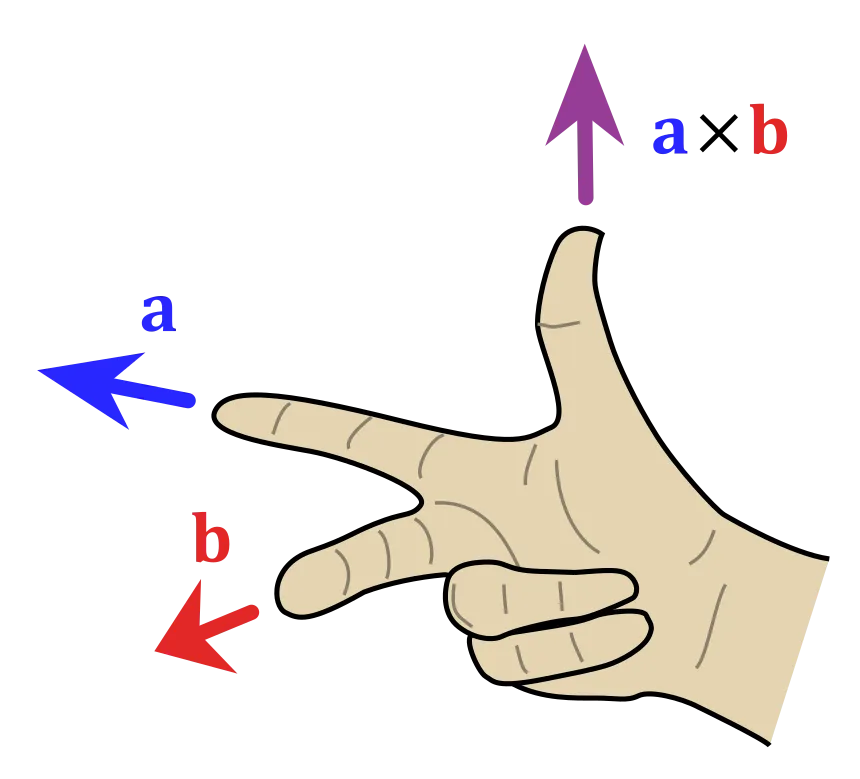
\includegraphics[width=.9\linewidth]{./images/right-hand-rule-cross-product.png}
\end{center}

 \newpage

\section{Mathematical formulas}
\label{sec:org3273cd0}

\subsection{Trigonometric identities}
\label{sec:orge5d1097}

\subsubsection{Basic and Pythagorean identities}
\label{sec:org5ebc8cb}
\[\csc x = \frac{1}{\sin x}\]
\[\sec x = \frac{1}{\cos x}\]
\[\cot x = \frac{1}{\tan x}\]
\[\sin (-x) = - \sin x\]
\[\cos (-x) = \cos x\]
\[\tan (-x) = - \tan x\]
\[\tan x = \frac{\sin x}{\cos x}\]
\[\cot x = \frac{\cos x}{\sin x}\]
\[\sin^2 x + \cos^2 x = 1\]
\[\tan^2 x + 1 = \sec x\]
\[1 + \cot^2 x = \csc^2 x\]

\subsubsection{Angle sum and different identities}
\label{sec:org0efbfcd}
\[\sin(A \pm B) = \sin A \cos B \pm \cos A \sin B\]
\[\sin(A \pm B) = \cos A \cos B \mp \sin A \sin B\]
\[\tan(A \pm B) = \frac{\tan A \pm \tan B}{1 \mp \tan A \tan B}\]

\subsubsection{Double angle identities}
\label{sec:orga30fd65}
\[\sin 2A = 2 \sin A \cos A\]
\[\cos 2A = \cos^2 A - \sin^2 A = 2 \cos^2 A - 1 = 1 - 2 \sin^2 A\]
\[\tan 2A = \frac{2 \tan A}{1 - \tan^2 A}\]

\subsubsection{Half angle identities}
\label{sec:org8973bed}
\[\sin \left(\frac{x}{2} \right) = \pm \sqrt{\frac{1 - \cos x}{2}}\]
\[\cos \left(\frac{x}{2} \right) = \pm \sqrt{\frac{1 + \cos x}{2}}\]
\[\tan \left(\frac{x}{2} \right) = \pm \sqrt{\frac{1 - \cos x}{1 + \cos x}} = \frac{1 - \cos x}{\sin x} = \frac{\sin x}{1 + \cos x}\]

\[\sin^2 x = \frac{1}{2} \left[1 - \cos 2x \right]\]
\[\cos^2 x = \frac{1}{2} \left[1 + \cos 2x \right]\]
\[\tan^2 x = \frac{1 - \cos 2x}{1 + \cos 2x}\]

\subsubsection{Sum identities}
\label{sec:org776acd2}
\[\sin P + \sin Q = 2 \sin \frac{1}{2}(P + Q) \cos \frac{1}{2}(P - Q)\]
\[\sin P - \sin Q = 2 \cos \frac{1}{2}(P + Q) \sin \frac{1}{2}(P - Q)\]
\[\cos P + \cos Q = 2 \cos \frac{1}{2}(P + Q) \cos \frac{1}{2}(P - Q)\]
\[\cos P - \cos Q = - 2 \sin \frac{1}{2}(P + Q) \sin \frac{1}{2}(P - Q)\]

\subsection{Standard derivatives}
\label{sec:org1ab4fef}
\[\frac{d}{dx} \left(\arcsin x \right) = \frac{1}{\sqrt{1 - x^2}}\]
\[\frac{d}{dx} \left(\arccos x \right) = - \frac{1}{\sqrt{1 - x^2}}\]
\[\frac{d}{dx} \left(\arctan x \right) = \frac{1}{1 + x^2}\]
\[\frac{d}{dx} \left(\csc x \right) = - \csc x \cot x\]
\[\frac{d}{dx} \left(\sec x \right) = \sec x \tan x\]

\subsection{Standard integrals}
\label{sec:org408d814}
\[\int \frac{1}{x^2 + a^2} \, dx = \frac{1}{a} \arctan \left(\frac{x}{a} \right)\]
\[\int \frac{1}{\sqrt{a^2 - x^2}} \, dx = \arcsin \left(\frac{x}{a} \right)\]
\[\int \frac{1}{x^2 - a^2} \, dx = \frac{1}{2a} \ln \left|\frac{x - a}{x + a} \right|\]
\[\int \frac{1}{a^2 - x^2} \, dx = \frac{1}{2a} \ln \left|\frac{a + x}{a - x} \right|\]
\[\int \frac{1}{\sqrt{x^2 - a^2}} \, dx = \ln \left|\sqrt{x^2 - a^2} + x \right|\]
\[\int \tan x \, dx = \ln |\sec x|\]
\[\int \cot x \, dx = \ln |\sin x|\]
\[\int \csc x \, dx = - \ln |\csc x + \cot x|\]
\[\int \sec x \, dx = - \ln |\sec x + \tan x|\]

\section{Figuring out the motion of objects relative to an attached frame of reference}
\label{sec:org39b3437}
\begin{enumerate}
\item Look at the length of the line with respect to the new origin of the attached frame of reference.
\item If the length of the line is constant, as in it doesn't change with time, then the motion of the object is likely a circular motion.
\item To confirm if the object is truly in circular motion, look at the angle the object makes with the origin of the attached frame.
\item This angle can be derived from the angle of the object with respect to the origin in the absolute frame.
\item If the angle is variable, as in it changes with time, then the object is circular motion.
\item Otherwise, if the angle is constant and doesn't change with time, then the object is not moving at all in the attached frame of reference.
\end{enumerate}

\section{Determining the friction direction}
\label{sec:org4ab8fd9}
\begin{enumerate}
\item Get the relative velocity of the object with respect to the other object that it is in contact with, and hence experiencing friction due to that contact.
\item The friction direction will always be opposite in direction to the obtained relative velocity.
\end{enumerate}

\section{Steps to solve collision problems}
\label{sec:org2ad52e2}
\begin{enumerate}
\item Set coordinates of the direction parallel (\(\hat{e}_n\)) and perpendicular (\(\hat{e}_t\)) to the impact, i.e. express \(\hat{i}\) and \(\hat{j}\) in terms of \(\hat{e}_n\) and \(\hat{e}_t\).
\item Set the restitution equation in the direction parallel to the impact (\(\hat{e}_n\) direction).
\item The direction perpendicular to the impact (\(\hat{e}_t\) direction) has no net force, and hence there is no change in velocities in that direction.
\item Gravitational force is negligible during the collision as the impact forces are relatively large.
\item Analyse the directions of the impact force and constrains to find the direction in which the net force of the system is zero. Apply the conservation of linear momentum in that direction.
\end{enumerate}

\section{Steps to solve pulley problems}
\label{sec:org0a04034}
\begin{enumerate}
\item Break down the system into individual objects.
\item Set the kinetic equation for each object.
\[F = ma \quad \text{and} \quad M = I \alpha\]
\item Find the relationship between the accelerations, the work done, or the energies.
\item Solve all the equations.
\end{enumerate}
\end{document}
